
\section{Organisation of appendices}
\label{sec:organ_suppl}

In this supplementary, we first introduce in \cref{sec:continuous_process} an Ornstein Uhlenbeck process on function space (via finite marginals) along with several score approximations.
Then in \cref{sec:manifold_valued}, we show how this methodology extend to manifold-valued inputs or outputs.
Later in \cref{sec:inv_ndp}, we derive sufficient conditions for this introduced model to yield a group invariant process.
What's more in \cref{sec:app_conditional_sampling}, we study some conditional sampling schemes.
Eventually in \cref{app:experimental_details}, we give a thorough description of experimental settings along with additional empirical results.

\section{Ornstein Uhlenbeck on function space} \label{sec:continuous_process}

\subsection{Multivariate Ornstein-Uhlenbeck process}
\label{sec:multivariate_ou}

First, we aim to show that we can define a stochastic process on an infinite dimensional function space, by defining the joint finite marginals $\v{Y}(x)$ as the solution of a multidimensional Ornstein-Uhlenbeck process.
In particular, for any set of input $x = (x_1, \cdots, x_k) \in \c{X}^k$, we define the joint marginal as the solution of the following SDE \begin{equation}\label{eq:app_forward_SDE_sp} \end{equation}

\begin{proposition}{\parencite{phillips2022spectral}}{} \label{prop:mOU} We assume we are given a data process $(\v{Y_}0(x))_{x \in \c{X}}$ and we denote by $\mathbf{G} \sim \mathrm{GP}(0, k)$ a Gaussian process with zero mean and covariance.
	Then let's define $$\v{Y_t} \triangleq e^{-\frac{1}{2}\cdot \int_{s=0}^t \beta_s ds} ~\v{Y_}0 + \left(1 - e^{-\frac{1}{2}\cdot \int_{s=0}^t \beta_s ds} \right) m + \left(1 - e^{-\int_{s=0}^t \beta_s ds} \right)^{1/2} \mathbf{G}.
	$$
	Then $(\v{Y_t}(x))_{x \in \c{X}}$ is a stochastic process (by virtue of being a linear combination of stochastic processes).
	We thus have that $\v{Y_t} xrightarrow[t \rightarrow 0]{a.s.
			} \v{Y_}0$ and $\v{Y_t} xrightarrow[t \rightarrow \infty]{a.s.} \v{Y_}\infty$ with $\v{Y_}\infty \sim \mathrm{GP}(m, k)$, so effectively $(\v{Y_t}(x))_{t \in \R_+, x \in \c{X}}$ interpolates between the data process and this limiting Gaussian process.
	Additionally, $\c{L}({\v{Y}}_t|{\v{Y}}_0=y_0) = \mathrm{GP}(m_t, K_t)$ with $m_t = e^{-\frac{1}{2}\cdot \int_{s=0}^t \beta_s ds} ~y_0 + \left(1 - e^{-\frac{1}{2}\cdot \int_{s=0}^t \beta_s ds} \right) m $ and $\Sigma_t = \left(1 - e^{-\int_{s=0}^t \beta_s ds} \right) {K}$.
	Furthermore, $(\v{Y_t}(x))_{t \in \R_+, x \in \c{X}}$ is the solution of the SDE in \eqref{eq:app_forward_SDE_sp}.
\end{proposition}

\begin{proof}
	We aim to compute the mean and covariance of the process $(\v{Y_t})_{t \geq 0}$ described by the SDE \eqref{eq:forward_SDE_sp}.
	First let's recall the time evolution of the mean and covariance of the solution from a multivariate Ornstein-Uhlenbeck process given by \begin{equation} \mathrm{d} \v{Y_t} = f(\v{Y_t}, t) \mathrm{d} t + L(\v{Y_t}, t) \mathrm{d} \v{B_t}.
	\end{equation}
	We know that the time evolution of the mean and the covariance are given respectively by \textcite{sarkka2019Applied} \begin{align} \frac{\mathrm{d} m_t}{\mathrm{d} t} & = \E[f(\v{Y_t}, t)] \\ \frac{\mathrm{d} \Sigma_t}{\mathrm{d} t} &= \E[f(\v{Y_t}, t) (m_t - \v{Y_t})^\top] + \E[(m_t - \v{Y_t}) f(\v{Y_t}, t)^\top ] + \E[L(\v{Y_t}, t) L(\v{Y_t}, t)^\top ].
	\end{align}
	Plugging in the drift $f(\v{Y_t}, t) = 1/2 \cdot (m - \v{Y_t}) \beta_t$ and diffusion term $L(\v{Y_t}, t) = \sqrt{\beta_t {K}}$ from \eqref{eq:forward_SDE_sp}, we get \begin{align} \frac{\mathrm{d} m_t}{\mathrm{d} t} & = 1/2 \cdot (m - \v{Y_t}) \beta_t \\ \frac{\mathrm{d} \Sigma_t}{\mathrm{d} t} &= \beta_t \left[ {K} -\Sigma_t \right].
	\end{align}
	Solving these two ODEs we get \begin{align} m_t &= e^{-\frac{1}{2}\cdot \int_{s=0}^t \beta_s ds} m_0 + \left(1 - e^{-\frac{1}{2}\cdot \int_{s=0}^t \beta_s ds} \right) m \\ \end{align} with $m_0 \triangleq \E[\v{Y_}0]$ and $\Sigma_0 \triangleq \mathrm{Cov}[\v{Y_}0]$.

	Now let's compute the first two moments of $(\v{Y_t}(x))_{x \in \c{X}}$.
	We have \begin{align} \E[\v{Y_t}] &= \E \left[ e^{-\frac{1}{2}\cdot \int_{s=0}^t \beta_s ds} ~\v{Y_}0 + \left(1 - e^{-\frac{1}{2}\cdot \int_{s=0}^t \beta_s ds} \right) m + \left(1 - e^{-\frac{1}{2}\cdot \int_{s=0}^t \beta_s ds} \right) \mathbf{G} \right] \\ &= e^{-\frac{1}{2}\cdot \int_{s=0}^t \beta_s ds} m_0 + \left(1 - e^{-\frac{1}{2}\cdot \int_{s=0}^t \beta_s ds} \right) m \\ &= m_t \end{align} \begin{align} \mathrm{Cov}[\v{Y_t}] & = \mathrm{Cov}\left[e^{-\frac{1}{2}\cdot \int_{s=0}^t \beta_s ds} ~\v{Y_}0\right] + \mathrm{Cov}\left[\left(1 - e^{- \int_{s=0}^t \beta_s ds} \right)^{1/2} \mathbf{G}\right] \\ &= e^{- \int_{s=0}^t \beta_s ds} ~\Sigma_0 + \left(1 - e^{- \int_{s=0}^t \beta_s ds} \right) {K} \\ &= {K} + e^{-\int_{s=0}^t \beta_s ds} \left( \Sigma_0 - {K} \right) \\ &= \Sigma_t .
	\end{align}
\end{proof}

\subsection{Conditional score}
\label{sec:multivariate_ou_score}
Hence, condition on ${\v{Y}}_0$ the score is the gradient of the log Gaussian characterised by mean $m_{t|0} = e^{-\frac{1}{2} B(t)} \v{Y_}0$ and $\Sigma_{t|0} = (1 - e^{-B(t)}) \mathrm{K}$ with $B(t) = \int_{0}^t \beta(s) ds$ which can be derived from the above marginal mean and covariance with $m_0 = \v{Y_}0$ and $\Sigma_0 = 0$.
\begin{align}
	\nabla_{{\v{Y}}_t} \log p_{t}({\v{Y}}_t| \v{Y_}0)
	 & = \nabla_{{\v{Y}}_t} \log \c{N}\left({\v{Y}}_t | m_{t|0}, \Sigma_{t|0} \right)                \\
	 & = \nabla_{{\v{Y}}_t} - 1/2 (\v{Y_t} - m_{t|0})^\top \Sigma_{t|0}^{-1} (\v{Y_t} - m_{t|0}) + c \\
	 & = - \Sigma_{t|0}^{-1} (\v{Y_t} - m_{t|0})                                                     \\
	 & = - \mathrm{L}_{t|0}^{-\top} \mathrm{L}_{t|0}^{-1} \mathrm{L}_{t|0} \epsilon                  \\
	 & = - \mathrm{L}_{t|0}^{-\top} \epsilon
\end{align}
where $\mathrm{L}_{t|0}$ denotes the Cholesky decomposition of $\Sigma_{t|0}=\mathrm{L}_{t|0} \mathrm{L}_{t|0}^\top$, and $\v{Y_t} = m_{t|0} + \mathrm{L}_{t|0} \epsilon$.

Then we can plugin our learnt (preconditioned) score into the backward SDE \ref{eq:backward_SDE_dupref2} which gives \begin{align}\label{eq:backward_SDE_sp_approx} \mathrm{d} \bar{\v{Y}}_t|x &= \left[-(m(x) - \bar{\v{Y}}_t)/2 + \mathrm{K}(x,x) \nabla_{\bar{\v{Y}}_t} \log p_{T-t}(t, x, \bar{\v{Y}}_t) \right] \mathrm{d} t + \sqrt{\beta_t \mathrm{K}(x,x)} \beta_t \mathrm{d} \v{B_t} \end{align}

\subsection{Several score parametrisations} \label{sec:app_parameterisation}

In this section, we discuss several parametrisations of the neural network and the objective.

For the sake of versatility, we opt to employ the symbol $D_\theta$ for the network instead of $s_\theta$ as mentioned in the primary text, as it allows us to approximate not only the score but also other quantities from which the score can be derived.
In full generality, we use a residual connection, weighted by ${c}_{\text{out}}, {c}_{\text{skip}}: \R \rightarrow \R$, to parameterise the network \begin{align} D_\theta(t, \v{Y}_t) = c_{\text{skip}}(t) \v{Y}_t + c_{\text{out}}(t) F_\theta(t, \v{Y}_t).
\end{align}
We recall that the input to the network is time $t$, and the noised vector $\v{Y}_t = \v{\mu}_{t|0} + \v{n}$, where $\v{\mu}_{t|0} = \textrm{e}^{-B(t)/2} \v{Y}_0$ and $\v{n} \sim \c{N}(0, \Sigma_{t|0})$ with $\Sigma_{t|0} = (1 - \textrm{e}^{-B(t)}) K$.
The gram matrix $K$ corresponds to $k(X, X)$ with $k$ the limiting kernel.
We denote by $\mathrm{L}_{t|0}$ and $\mathrm{S}$ respectively the Cholesky decomposition of $\Sigma_{t|0}=\mathrm{L}_{t|0} \mathrm{L}_{t|0}^\top$ and $\mathrm{K} = \mathrm{S} \mathrm{S}^\top$.

The denoising score matching loss weighted by $\Lambda(t)$ is given by \begin{align} \label{eq:app:loss} \c{L}(\theta) = \mathbb{E} \left[\| {D}_\theta(t, \v{Y}_t) - \nabla_{{\v{Y}}_t} \log p_{t}(\v{Y}_t| \v{Y}_0)\|_{\Lambda(t)}^2 \right] \end{align}

\begin{table}[] \centering \small \begin{tabular}{lllll} \toprule                 & No precond.
                                                & Precond. $K$                                & Precond. $S^\top$                         & Predict $\v{Y}_0$                   \\
               \midrule
               $c_\text{skip}$                  & 0                                           & 0                                         & 0                               & 1 \\
               $c_\text{out}$                   & $(\sigma_{t|0} + 10^{-3})^{-1}$             & $(\sigma_{t|0} + 10^{-3})^{-1}$           & $(\sigma_{t|0} + 10^{-3})^{-1}$ & 1 \\
               Loss                             & $\|\sigma_{t|0}
               S^\top D_{\theta} + \v{z}\|_2^2$ & $\|\sigma_{t|0} D_{\theta} + S \v{z}\|_2^2$ & $\|\sigma_{t|0} D_{\theta} + \v{z}\|_2^2$ & $\|D_{\theta} - \v{Y}_0\|^2_2$      \\ $K \nabla \log p_t$ & $K D_\theta$ & $D_\theta$ & $ S D_\theta $ & $-\Sigma_{t|0}^{-1}(\v{Y}_t - \textrm{e}^{{-}\frac{B(t)}{2}} D_\theta)$ \\ \bottomrule\end{tabular} \caption{Summary of different score parametrisations as well as the values for $c_{\text{skip}}$ and $c_{\text{out}}$ that we found to be optimal, based on the recommendation from \textcite[Appendix B.6]{karras2022Elucidatinga}.
	}\label{tab:app:score-param}
\end{table}

\paragraph{No preconditioning}

By reparametrisation, let $\v{Y}_t = \v{\mu}_{t|0} + L_{t|0} \v{z}$, where $\v{z} \sim \c{N}(\v{0}, \m{I})$, the loss from \cref{eq:app:loss} can be written as \begin{align} \c{L}(\theta) &= \mathbb{E}\left[ \| D_\theta(t, \v{Y}_t) + \Sigma_{t|0}^{-1} (\v{Y}_t - \v{\mu}_{t|0}) \|^2_{\Lambda(t)} \right] \\ &= \mathbb{E}\left[ \| D_\theta(t, \v{Y}_t) + \Sigma_{t|0}^{-1} L_{t|0}\v{z} \|^2_{\Lambda(t)} \right] \\ &= \mathbb{E}\left[ \| D_\theta(t, \v{Y}_t) + L_{t|0}^{-\top}\v{z} \|^2_{\Lambda(t)} \right] \\ \end{align} Choosing $\Lambda(t) = \Sigma_{t|0} = L_{t|0}L_{t|0}^\top$ we obtain \begin{align} \c{L}(\theta) & = \mathbb{E}\left[ \| L_{t|0}^\top D_\theta(t, \v{Y}_t) + \v{z} \|^2_{2} \right] \\ &= \mathbb{E}\left[ \| \sigma_{t|0} S^\top D_\theta(t, \v{Y}_t) + \v{z} \|^2_{2} \right].
\end{align}

\paragraph{Preconditioning by ${K}$}

Alternatively, one can train the neural network to approximate the preconditioned score $D_\theta \approx \m{K} \nabla_{\v{Y}_t} \log p_t(\v{Y}_t | \v{Y}_0)$.
The loss, weighted by $\Lambda = \sigma_{t|0}^2\m{I}$, is then given by \begin{align} \c{L}(\theta) & = \mathbb{E}\left[ \| D_\theta(t, \v{Y}_t) + {K}\,L_{t|0}^{-\top}\v{z} \|^2_{\Lambda(t)} \right] \\ &= \mathbb{E}\left[ \| D_\theta(t, \v{Y}_t) + \sigma_{t|0}^{-1}{S}\v{z} \|^2_{\Lambda(t)} \right] \\ &= \mathbb{E}\left[ \| \sigma_{t|0}D_\theta(t, \v{Y}_t) + {S}\v{z} \|^2_{2} \right].
\end{align}

\paragraph{Precondition by $S^\top$}
A variation of the previous one, is to precondition the score by the transpose Cholesky of the limiting kernel gram matrix, such that $ D_\theta \approx {S}^\top \nabla_{\v{Y}_t} \log p_t(\v{Y}_t | \v{Y}_0) $ .

The loss, weighted by $\Lambda = \sigma_{t|0}^2\m{I}$, becomes \begin{align} \c{L}(\theta) & = \mathbb{E}\left[ \| D_\theta(t, \v{Y}_t) + {S}^\top\,L_{t|0}^{-\top}\v{z} \|^2_{\Lambda(t)} \right] \\ &= \mathbb{E}\left[ \| D_\theta(t, \v{Y}_t) + \sigma_{t|0}^{-1}\v{z} \|^2_{\Lambda(t)} \right] \\ &= \mathbb{E}\left[ \| \sigma_{t|0}D_\theta(t, \v{Y}_t) + \v{z} \|^2_{2} \right].
\end{align}

\paragraph{Predicting $\v{Y}_0$}

Finally, an alternative strategy is to predict $\v{Y}_0$ from a noised version $\v{Y}_t$.
In this case, the loss takes the simple form $$ \c{L}(\theta) = \mathbb{E}\left[\| D_\theta(t, \v{Y}_t) - \v{Y}_0 \|^2_2\right].
$$
The score can be computed from the network's prediction following
\begin{align}
	\nabla \log p_t(\v{Y}_t | \v{Y}_0) & = -\Sigma_{t|0}^{-1}(\v{Y}_t - \v{\mu}_{t|0})                  \\
	                                   & = -\Sigma_{t|0}^{-1}(\v{Y}_t - \textrm{e}^{-B(t)/2} \v{Y}_0)   \\
	                                   & \approx -\Sigma_{t|0}^{-1}\left(\v{Y}_t - \textrm{e}^{-B(t)/2}
	D_\theta(t, \v{Y}_t)\right)                                                                         \\\end{align}

\Cref{tab:app:score-param} summarises the different options for parametrising the score as well as the values for $c_{\text{skip}}$ and $c_{\text{out}}$ that we found to be optimal, based on the recommendation from \textcite[Appendix B.6]{karras2022Elucidatinga}.
In practice, we found the precondition by $K$ parametrisation to produce the best results, but we refer to \cref{fig:app:score-parametrization-ablation} for a more in-depth ablation study.

\subsection{Exact (marginal) score in Gaussian setting}
Interpolating between Gaussian processes $GP(m_0, \Sigma_0)$ and $GP(m, \mathrm{K})$ \begin{align} \mathrm{K} \nabla_{\bar{\v{Y}}_t} \log p_t(\v{Y_t}) &= - \mathrm{K} \Sigma_{t}^{-1} (\v{Y_t} - m_{t}) \\ &= - \mathrm{K} [\mathrm{K} + e^{-\int_{s=0}^t \beta_s ds} \left( \Sigma_0 - \mathrm{K} \right)]^{-1} (\v{Y_t} - m_{t}) \\ &= - \mathrm{K} ({\mathrm{L}_t}{L_t}^\top)^{-1} (\v{Y_t} - m_{t}) \\ &= - \mathrm{K} {{\mathrm{L}_t}^\top}^{-1} {\mathrm{L}_t}^{-1}\textbf{} (\v{Y_t} - m_{t}) \\ \end{align} with $\Sigma_t = \mathrm{K} + e^{-\int_{s=0}^t \beta_s ds} \left( \Sigma_0 - \mathrm{K} \right) = {\mathrm{L}_t}{\mathrm{L}_t}^\top$ obtained via Cholesky decomposition.

\subsection{Langevin dynamics}
Under mild assumptions on $\nabla \log p_{T-t}$ \parencite{durmus:moulines:2016} the following SDE \begin{equation}\label{eq:app_langevin} \mathrm{d} \v{Y_s} = \tfrac{1}{2} \mathrm{K} \nabla \log p_{T-t}(\v{Y_s}) \mathrm{d} s + \sqrt{\mathrm{K}} \mathrm{d} \v{B_s} \end{equation} admits a solution $(\v{Y_s})_{s\ge0}$ whose law $\c{L}(\v{Y_s})$ converges with geometric rate to $p_{T-t}$ for any invertible matrix $\mathrm{K}$.

\subsection{Likelihood evaluation}

Similarly to \textcite{song2020score}, we can derive a deterministic process which has the same marginal density as the SDE \eqref{eq:forward_SDE_sp}, which is given by the following Ordinary Differential Equation (ODE)---referred as the probability flow ODE \begin{align} \label{eq:probability_flow_ode} \mathrm{d} \begin{pmatrix} \hspace{2.2em} \v{Y}_t(x) \\ \log p_t(\v{Y}_t(x)) \end{pmatrix} = \begin{pmatrix} \hspace{2em} \tfrac{1}{2} \left\{ m(x) - \v{Y}_t(x) - \mathrm{K}(x,x) \nabla \log p_t( \v{Y}_t(x)) \right\} \beta_t \\ - \tfrac{1}{2} \dive \left\{ m(x) - \v{Y}_t(x) - \mathrm{K}(x,x) \nabla \log p_t( \v{Y}_t(x)) \right\} \beta_t \end{pmatrix} \mathrm{d} t .
\end{align}

Once the score network is learnt, we can thus use it in conjunction with an ODE solver to compute the likelihood of the model.

\subsection{Discussion consistency}
\label{sec:consistency}
So far we have defined a generative model over functions via its finite marginals $\bar{\v{Y}}^\theta_T(x)$.
These finite marginals were to arise from a stochastic process if, as per the Kolmogorov extension theorem \parencite{oksendal2003stochastic}, they satisfy \emph{exchangeability} and \emph{consistency} conditions.
Exchangeability can be satisfied by parametrising the score network such that the score network is equivariant w.r.t\ permutation, i.e.\ $\mathbf{s}_\theta(t, \sigma \circ x, \sigma \circ {y}) = \sigma \circ \mathbf{s}_\theta(t, x, {y})$ for any $\sigma \in \Sigma_n$.
Additionally, we have that the noising process $({\v{Y}}_t(x))_{x \in \c{X}}$ is trivially consistent for any $t \in \R_+$ since it is a stochastic process as per \cref{prop:mOU}, and consequently so is the (true) time-reversal $(\bar{\v{Y}}_t(x))_{x \in \c{X}}$.
Yet, when approximating the score $\mathbf{s}_\theta \approx \nabla \log p_{t}$, we lose the consistency over the generative process $\bar{\v{Y}}^\theta_t(x)$ as the constraint on the score network is non trivial to satisfy.
This is actually a really strong constraint on the model class, and as soon as one goes beyond linearity (of the posterior w.r.t.\ the context set), it is non trivial to enforce without directly parameterising a stochastic process, e.g.\ as extcite{phillips2022spectral}.
There thus seems to be a strong trade-off between satisfying consistency, and the model's ability to fit complex process and scale to large datasets.

\section{Manifold-valued diffusion process}
\label{sec:manifold_valued}

\subsection{Manifold-valued inputs}
\label{sec:manifold_valued_input}

In the main text we dealt with a simplified case of tensor fields where the tensor fields are over Euclidean space.
Nevertheless, it is certainly possible to apply our methods to these settings.
Significant work has been done on performing convolutions on feature fields on generic manifolds (a superset of tensor fields on generic manifolds), core references being \cite{cohen2021equivariant} for the case of homogeneous spaces and \cite{weiler2021coordinate} for more general Riemannian manifolds.
We recommend these as excellent mathematical introductions to the topic and build on them to describe how to formulate diffusion models over these spaces.

\textbf{Tensor fields as sections of bundles.}
Formally the fields we are interested in modelling are sections $\sigma$ of associated tensor bundles of the principle $G$-bundle on a manifold $M$.
We shall denote such a bundle $BM$ and the space of sections $\Gamma(BM)$.
The goal, therefore, is to model \textit{random elements} from this space of sections.
For a clear understanding of this definition, please see \textcite[pages 73-95]{weiler2021coordinate} for an introduction suitable to ML audiences.
Prior work looking at this setting is \cite{hutchinson2021vector} where they construct Gaussian Processes over tensor fields on manifolds.

\textbf{Stochastic processes on spaces of sections.}
Given we can see sections as maps $\sigma: M \to BM$, where an element in $BM$ is a tuple $(m, b)$, $m$ in the base manifold and $b$ in the typical fibre, alongside the condition that the composition of the projection $\operatorname{proj}_i: (m, b)\mapsto m$ with the section is the identity, $\operatorname{proj}_i \circ \sigma = \operatorname{Id}$ it is clear we can see distribution over sections as stochastic processes with index set the manifold $M$, and output space a point in the bundle $BM$, with the projection condition satisfied.
The projection onto finite marginals, i.e.\ a finite set of points in the manifold, is defined as $\pi_{m_1, .
		.., m_n}(\sigma) = (\sigma(m_1), ..., \sigma(m_n))$.

\textbf{Noising process.}
To define a noising process over these marginals, we can use Gaussian Processes defined in \cite{hutchinson2021vector} over the tensor fields.
The convergence results of \textcite{phillips2022spectral} hold still, and so using these Gaussian Processes as noising processes on the marginals also defines a noising process on the whole section.

\textbf{Reverse process.}
The results of \cite{cattiaux2021time} are extremely general and continue to hold in this case of SDEs on the space of sections.
Note we don't actually need this to be the case, we can just work with the reverse process on the marginals themselves, which are much simpler objects.
It is good to know that it is a valid process on full sections though should one want to try and parameterise a score function on the whole section akin to some other infinite-dimension diffusion models.

\textbf{Score function.}
The last thing to do therefore is parameterise the score function on the marginals.
If we were trying to parameterise the score function over the \textit{whole} section at once (akin to a number of other works on infinite dimension diffusions), this could present some problems in enforcing the smoothness of the score function.
As we only deal with the score function on a finite set of marginals, however, we need not deal with this issue and this presents a distinct advantage in simplicity for our approach.
All we need to do is pick a way of numerically representing points on the manifold and b) pick a basis for the tangent space of each point on the manifold.
This lets us represent elements from the tangent space numerically, and therefore also elements from tensor space at each point numerically as well.
This done, we can feed these to a neural network to learn to output a numerical representation of the score on the same basis at each point.

\subsection{Manifold-valued outputs}
\label{sec:manifold_valued_output}
In the setting, where one aim to model a stochastic process with manifold codomain ${\v{Y}}_t(x) = ({\v{Y}}_t(x_1), \cdots, {\v{Y}}_t(x_n)) \in \c{M}^n$, things are less trivial as manifolds do not have a vector space structure which is necessary to define Gaussian processes.
Fortunately, We can still target a know distribution marginally independently on each marginal, since this is well defined, and as such revert to the Riemannian diffusion models introduced in \textcite{debortoli2021neurips} with $n$ independent Langevin noising processes \begin{equation} \label{eq:forward_SDE_manifold} \mathrm{d} {\v{Y}}_t(x_k) = - \tfrac{1}{2} \nabla U({\v{Y}}_t(x_k))~\beta_t \mathrm{d} t + \sqrt{\beta_t } \mathrm{d} \v{B}_t^\c{M} .
\end{equation}
are applied to each marginal.
Hence in the limit $t \rightarrow \infty$, ${\v{Y}}_t(x)$ has density (assuming it exists) which factors as $dp / d \mathrm{Vol}_\c{M}((y(x_1), \cdots, y(x_n))) \propto \prod_k e^{-U(y(x_n)))}$.
For compact manifolds, we can target the uniform distribution by setting $U(x)=0$.
The reverse time process will have correlation between different marginals, and so the score function still needs to be a function of all the points in the marginal of interest.

\section{Invariant neural diffusion processes}
\label{sec:inv_ndp}

\subsection{$\mathrm{E}(n)$-equivariant kernels}
\label{sec:en_equiv_kernels}

A kernel $k: \R^d \times \R^d \rightarrow \R^{d\times d}$ is equivariant if it satisfies the following constraints: (a) $k$ is \emph{stationnary}, that is if for all $x, x' \in \R^n$

\begin{align} k(x, x') = k(x - x') \triangleq \tilde{k}(x - x') \end{align} and if (b) it satisfies the \emph{angular constraint} for any $h \in H$ \begin{align} k(h x, h x') = \rho(h) k(x, x') \rho(h)^\top.
\end{align}

A trivial example of such an equivariant kernel is the diagonal kernel $k(x,x') = k_0(x, x') \mathrm{I}$ \parencite{holderrieth2021equivariant}, with $k_0$ stationnary.
This kernel can be understood has having $d$ independent Gaussian process uni-dimensional output, that is, there is no inter-dimensional correlation.

Less trivial examples, are the $\mathrm{E}(n)$ equivariant kernels proposed in \textcite{macedo2010learning}.
Namely curl-free and divergence-free kernels, allowing for instance to model electric or magnetic fields.
Formally we have $k_\mathrm{curl} = k_0 A$ and $k_\mathrm{div} = k_0 B$ with $k_0$ stationary, e.g.\ squared exponential kernel $k_0(x, x') = \sigma^2 \exp\left(\frac{\| x - x' \|^2}{2 l^2} \right)$, and $A$ and $B$ given by \begin{align} A(x, x') = \mathrm{I} - \frac{(x - x')(x - x')^\top}{l^2} \end{align} \begin{align} B(x, x') = \frac{(x - x')(x - x')^\top}{l^2} + \left( n -1 - \frac{\|x - x' \|^2}{l^2} \right) \mathrm{I}.
\end{align}
See \textcite[Appendix C, ][]{holderrieth2021equivariant} for a proof.

\subsection{Proof of \cref{prop:inv_prior}}
\label{sec:proof_inv_prior}
Below we give two proofs for the group invariance of the generative process, one via the probability flow ODE and one directly via Fokker-Planck.

\begin{proof}
	The reverse probability flow associated with the forward SDE \eqref{eq:forward_SDE_sp} with approximate score $\mathbf{s}_\theta(t, \cdot) \approx \nabla \log p_t$ is given by

	\begin{align} \label{eq:backward_ODE_sp} \mathrm{d} \bar{\v{Y}}_t|x &= \tfrac{1}{2} \left[-m(x) + \bar{\v{Y}}_t + \mathrm{K}(x,x) \mathbf{s}_\theta(T - t, x, \bar{\v{Y}}_t) \right] \mathrm{d} t \\ & \triangleq b_{\text{ODE}}(t, x, \bar{\v{Y}}_t) \mathrm{d} t \end{align} This ODE induces a flow $\phi^b_t: X^n \times Y^n \rightarrow \mathrm{T}Y^n$ for a given integration time $t$, which is said to be $G$-equivariant if the vector field is $G-$equivariant itself, i.e.\ $b(t, g\cdot x, \rho(g) \bar{\v{Y}}_t) = \rho(g) b(t, x, \bar{\v{Y}}_t)$.
	We have that for any $g \in G$ \begin{align} b_{\text{ODE}}(t, g\cdot x, \rho(g) \bar{\v{Y}}_t) &= \tfrac{1}{2} \left[ -m(g \cdot x) + \rho(g) \v{Y}_t + \mathrm{K}(g \cdot x,g \cdot x) ~\mathbf{s}_\theta(t, g \cdot x, \rho(g) \bar{\v{Y}}_t) \right] \\ &\overset{(1)}{=} \tfrac{1}{2} \left[-\rho(g)m(x) + \rho(g) \v{Y}_t + \rho(g) \mathrm{K}(x,x)\rho(g)^\top ~\mathbf{s}_\theta(t, g \cdot x, \rho(g) \bar{\v{Y}}_t) \right] \\ &\overset{(2)}{=} \tfrac{1}{2} \left[-\rho(g)m(x) + \rho(g) \v{Y}_t + \rho(g) \mathrm{K}(x,x)\rho(g)^\top \rho(g) ~\mathbf{s}_\theta(t, x, \bar{\v{Y}}_t) \right] \\ &\overset{(3)}{=} \tfrac{1}{2} \rho(g) \left[-m(x) + \v{Y}_t + \mathrm{K}(x,x) ~\mathbf{s}_\theta(t, x, \bar{\v{Y}}_t) \right] \\ &\overset{}{=} \rho(g) b_{\text{ODE}}(t, x, \bar{\v{Y}}_t) \end{align} with (1) from the $G$-invariant prior GP conditions on $m$ and $k$, (2) assuming that the score network is $G$-equivariant and (3) assuming that $\rho(g) \in O(n)$.
	To prove the opposite direction, we can simply follow these computations backwards.
	Finally, we know that with a $G$-invariant probability measure $p_{\textup{ref}}$ and $G$-equivariant map $\phi$, the pushforward probability measure $p_{\textup{ref}}^{-1} \circ \phi$ is also $G$-invariant \parencite{kohler2020equivariant,papamakarios2019normalizing}.
	Assuming a $G$-invariant prior GP, and a $G$-equivariant score network, we thus have that the generative model from \cref{sec:diffusion_sp} defines marginals that are $G$-invariant.
\end{proof}

\begin{proof}
	The reverse SDE associated of the forward SDE \eqref{eq:forward_SDE_sp} with approximate score $\mathbf{s}_\theta(t, \cdot) \approx \nabla \log p_t$ is given by \begin{align}\label{eq:backward_SDE_sp_approx2} \mathrm{d} \bar{\v{Y}}_t|x & = \left[-(m(x) - \bar{\v{Y}}_t)/2 + \mathrm{K}(x,x) \mathbf{s}_\theta(T - t, x, \bar{\v{Y}}_t) \right] \mathrm{d} t + \sqrt{\beta_t \mathrm{K}(x,x)} \mathrm{d} \v{B}_t \\ &\triangleq b_{\text{SDE}}(t, x, \bar{\v{Y}}_t) \mathrm{d} t + \Sigma^{1/2}(t, x) ~\mathrm{d} \v{B}_t.
	\end{align}

	As for the probability flow drift $b_{\text{ODE}}$, we have that $b_{\text{SDE}}$ is similarly $G$-equivariant, that is $b_{\text{SDE}}(t, g\cdot x, \rho(g) \bar{\v{Y}}_t) = \rho(g) b_{\text{SDE}}(t, x, \bar{\v{Y}}_t)$ for any $g \in G$.
	Additionally, we have that diffusion matrix is also $G$-equivariant as for any $g \in G$ we have $\Sigma(t, g \cdot x) = \beta_t \mathrm{K}(g \cdot x, g \cdot x) = \beta_t \rho(g) \mathrm{K}(x, x) \rho(g)^\top = \rho(g) \Sigma(t, x) \rho(g)^\top$ since $\mathrm{K}$ is the gram matrix of an $G$-equivariant kernel $k$.

	Additionally assuming that $b_{\text{SDE}}$ and $\Sigma$ are bounded, \textcite[Proposition 3.6,][]{yim2023se} says that the distribution of $\bar{\v{Y}}_t$ is $G$-invariant, and in in particular $\mathcal{L}(\bar{\v{Y}}_0)$.

\end{proof}

\subsection{Equivariant posterior maps}
\label{sec:equiv_posterior}
\label{sec:proof_equiv_posterior}

\def\phiA{\phi_{*, \c{A}}}
\def\iso{\operatorname{Isom}}

\begin{theorem}[Invariant prior stochastic process implies an equivariant posterior map]
	Using the language of \textcite{weiler2021coordinate} our tensor fields are sections of an associated vector bundle $\c{A}$ of a manifold $M$ with a $G$ structure.
	Let $\iso_{GM}$ be the group of $G$-structure preserving isometries on $M$.
	The action of this group on a section of the bundle $f \in \Gamma(\c{A})$ is given by \[ \phi \triangleright f := \phiA \circ f \circ \phi^{-1} \] \cite{weiler2021coordinate}.
	Let $f \sim P$, $P$ a distribution over the space of section.
	Let $\phi \triangleright P$ be the law of of $\phi \triangleright f$.
	Let $\mu_x = \c{L}(f(x)) = {\pi_x}_\# P$, the law of $f$ evaluated at a point, where $\pi_x$ is the canonical projection operator onto the marginal at $x$, $\#$ the pushforward operator in the measure theory sense, $x\in M$ and $y$ is in the fibre of the associated bundle.
	Let $\mu_x^{x', y} = \c{L}(f(x) | f(x') = y') = {\pi_x} \mu^{x', y'} = {\pi_x}_{\#} \c{L}(f | f(x') = y')$, the conditional law of the process when given $f(x') = y'$.

	Assume that the prior is invariant under the action of $\iso_{GM}$, i.e. that \[\phi \triangleright \mu_x = \del{\phiA}_\# \mu_{\phi^{-1}(x)} = \mu_x\]

	Then the conditional measures are equivariant, in the sense that \[\phi \triangleright \mu_x^{x', y'} = \del{\phiA}_\#\mu_{\phi^{-1}(x)}^{x',y'} = \mu_x^{\phi^{-1}(x), \phiA(y)} = \mu_x^{\phi \triangleright (x', y')}\]

\end{theorem}

\begin{proof} \(\forall A, B\) test functions, $\phi \in \iso_{GM}$, \begin{align*} \E\sbr{B\del{f(x')}A\del{(\phi \triangleright f)(x)} } & = \E\sbr{ B\del{f(x')} A\del{{\phiA \circ f \circ \phi^{-1}}(x)}} \\ & = \E\sbr{ B\del{f(x')} \E\sbrvert{A\del{\phiA\del{F(\phi^{-1}(x))}}}{F(x')}} \\ & = \E\sbr{ B\del{f(x')} \int{ A(y) \del{\phiA}_\# \mu_{\phi^{-1}(x)}^{x', f(x')}}(\mathrm{d}y)} \\ & = \int{ B\del{y'} \int{ A(y) \del{\phiA}_\# \mu_{\phi^{-1}(x)}^{x', f(x')}}(\mathrm{d}y) \mu_{x'}(\mathrm{d}y')} \\ & = \int{ B\del{y'} \int{ A(y) \del{\phi \triangleright \mu_{x}^{x', f(x')}}}(\mathrm{d}y) \mu_{x'}(\mathrm{d}y')} \\ \end{align*} By invariance this quantity is also equal to \begin{align*} \E\sbr{B\del{(\phi^{-1}\triangleright f)(x')} A((\phi^{-1}\triangleright \phi \triangleright f)(x))} & = \E\sbr{B\del{(\phi^{-1}\triangleright f)(x')} \E\sbrvert{ A(f(x))}{B\del{(\phi^{-1}\triangleright f)(x')}}} \\ & = \E\sbr{B\del{\phiA (f(\phi^{-1}(x')))} \sbrvert{ A(F(x))}{\phiA (f(\phi^{-1}(x')))}} \\ & = \E\sbr{B\del{\tau_{x', g}^{-1} F(gx')} \int{ A(y) \mu_x^{\phi(x'), \phiA^{-1}(y)}}}(\mathrm{d}y) \\ & = \int{B(y')\int{ A(y) \mu_x^{\phi\triangleright (x', y)}}}(\mathrm{d}y) \del{\phiA^{-1}}_\# \mu_{\phi(x')}(\mathrm{d}y') \\ & = \int{B(y')\int{ A(y) \mu_x^{\phi\triangleright (x', y)}}}(\mathrm{d}y) \del{\phi^{-1} \triangleright \mu_{x'}}(\mathrm{d}y') \\ \end{align*} Hence \begin{align*} \del{\phi \triangleright \mu_{x}^{x', f(x')}}(\mathrm{d}y) \mu_{x'}(\mathrm{d}y') = \mu_x^{\phi\triangleright (x', y)}(\mathrm{d}y) \del{\phi^{-1} \triangleright \mu_{x'}}(\mathrm{d}y') \end{align*} By the stated invariance \( \phi^{-1} \triangleright \mu_{x'} = \mu_{x'}\), hence \begin{align*} \del{\phi \triangleright \mu_{x}^{x', f(x')}}(\mathrm{d}y) = \mu_x^{\phi\triangleright (x', y)}(\mathrm{d}y) \;\text{a.e.
		}\;y'
	\end{align*}
	So \begin{align} \phi \triangleright \mu_{x}^{x', f(x')} = \mu_x^{\phi\triangleright (x', y)} \end{align} as desired.
\end{proof}

\section{Langevin corrector and the iterative procedure of \textsc{RePaint}~\parencite{lugmayr2022RePaint}}
\label{sec:app_conditional_sampling}

\subsection{Langevin sampling scheme}

Several previous schemes exist for conditional sampling from Diffusion models.
Two different types of conditional sampling exist.
Those that try to sample conditional on some part of the state space over which the diffusion model has been trained, such as in-painting or extrapolation tasks, and those that post-hoc attempt to condition on something outside the state space that the model has been trained on.

This first category is the one we are interested in, and in it we have: \begin{itemize} \item Replacement sampling \cite{song2020score}, where the reverse ODE or SDE is evolved but by fixing the conditioning data during the rollout.
	      This method does produce visually coherent sampling in some cases, but is not an exact conditional sampling method.
	\item SMC-based methods \cite{trippe2022Diffusion}, which are an exact method up to the particle filter assumption.
	      These can produce good results but can suffer from the usual SMC methods downsides on highly multi-model data such as particle diversity collapse.
	\item The {\textsc RePaint} scheme of \cite{lugmayr2022RePaint}.
	      While not originally proposed as an exact sampling scheme, we will show later that it can in fact be shown that this method is doing a specific instantiation of our newly proposed method, and is therefore exact.
	\item Amortisation methods, e.g. \textcite{phillips2022spectral}.
	      While they can be effective, these methods can never perform exact conditional sampling, by definition.
\end{itemize}

Our goal is to produce an exact sampling scheme that does not rely on SMC-based methods.
Instead, we base our method on Langevin dynamics.
If we have a score function trained over the state space $\v{x} = [\v{x}^c, \v{x}^*]$, where $\v{x}^c$ are the points we wish to condition on and $\v{x}_s$ points we wish to sample, we exploit the following score breakdown: \[\nabla_{\v{x}^*} \log p(\v{x}^*|\v{x}^c) = \nabla_{\v{x}^*} \log p([\v{x}^*, \v{x}^c]) - \nabla_{\v{x}^*} \log p(\v{x}^c) = \nabla_{\v{x}^*} \log p(\v{x})\] If we have access to the score on the joint variables, we, therefore, have access to the conditional score by simply only taking the gradient of the joint score for the variable we are not conditioning on.

Given we have learnt $s_\theta(t, \v{x}) \approx \nabla_{\v{x}}\log p_t(\v{x})$, we could use this to perform Langevin dynamics at $t=\epsilon$, some time very close to $0$.
Similar to \cite{song2019generative} however, this produces the twin issues of how to initialise the dynamics, given a random initialisation will start the sampler in a place where the score has been badly learnt, producing slow and inaccurate sampling.

Instead, we follow a scheme of tempered Langevin sampling detailed in \cref{alg:conditioning_langevin}.
Starting at $t=T$ we sample an initialisation of $\v{y}^*$ based on the reference distribution.
Progressing from $t=T$ towards $t=\epsilon$ we alternate between running a series of Lavgevin corrector steps to sample from the distribution $p_{t, \v{x}^*}(\v{y}^* | \v{y}^c)$, and a single backwards SDE step to sample from $p_{\v{x}}(\v{y}_{t-\gamma} | \v{y}_t)$ with a step size $\gamma$.
At each inner and outer step, we sample a noised version of the conditioning points $\v{y}^c$ based forward SDE applying noise to these context points, $p_{t, \v{x}^c}(\v{y}_t^c | \v{y}^c)$.
For the exactness of this scheme, all that matters is that at the end of the sampling scheme, we are sampling from $p_{\v{x}^*}(\v{y}^* | \v{y}^c)$ (up to the $\epsilon$ away from zero clipping of the SDE).
The rest of the scheme is designed to map from the initial sample at $t=T$ of $\v{y}^*$ to a viable sample through \textit{regions where the score has been learnt well}.

Given the noising scheme applied to the context points does not actually play into the theoretical exactness of the scheme, only the practical difficulty of staying near regions of well-learnt score, we could make a series of different choices for how to noise the context set at each step.

The choices that present themselves are \begin{enumerate} \item The initial scheme of sampling context noise from the SDE every inner and outer step.
	\item Only re-sampling the context noise every outer step, and keeping it fixed to this for each inner step associated with the outer step.
	\item Instead of sampling independent marginal noise at each outer step, sampling a single noising trajectory of the context set from the forward SDE and use this as the noise at each time.
	\item Perform no noising at all.
	      Effectively the replacement method with added Langevin sampling.
\end{enumerate}
These are illustrated in \cref{fig:noise_schemes}.
\begin{figure}
	\centering
	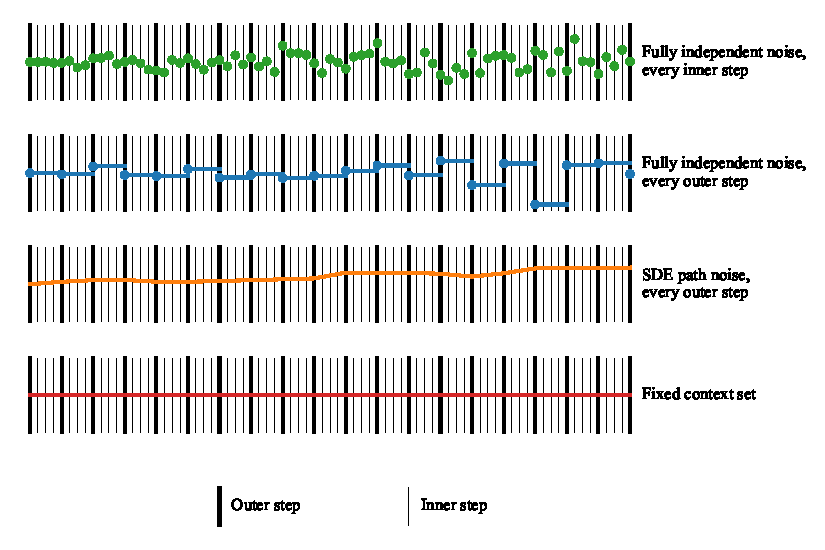
\includegraphics{images/geomndp/compare_noising_schemes.pdf}
	\caption{Comparison of different context noising schemes for the conditional sampling.}
	\label{fig:noise_schemes}
\end{figure}
The main trade-off of different schemes is the speed at which the noise can be sampled vs sample diversity.
In the Euclidean case, we have a closed form for the evolution of the marginal density of the context point under the forward SDE.
In this case sampling the noise at a given time is $\c{O}(1)$ cost.
On the other hand, in some instances such as nosing SDEs on general manifolds, we have to simulate this noise by discretising the forward SDE.
In this case, it is $\c{O}(n)$ cost, where $n$ is the number of discretisation steps in the SDE.
For $N$ outer steps and $I$ inner steps, the complexity of the different noising schemes is compared in \cref{tab:noise_comp}.
Note the conditional sampling scheme other than the noise sampling is $\c{O}(NI)$ complexity.

\begin{table}[]
	\centering
	\begin{tabular}{lrr}
		\toprule
		{\textsc Scheme}                              & {\textsc Closed-form noise} & {\textsc Simulated noise} \\
		\midrule
		{\textsc Re-sample noise at every inner step} & $\c{O}(NI)$                 & $\c{O}(N^2I^2)$           \\
		{\textsc Re-sample noise at every outer step} & $\c{O}(N)$                  & $\c{O}(N^2)$              \\
		{\textsc Sampling an SDE path on the context} & $\c{O}(N)$                  & $\c{O}(N)$                \\
		{\textsc No noise applied}                    & -                           & -                         \\
		\bottomrule
	\end{tabular}
	\caption{Comparison of complexity of different noise sampling schemes for the context set.}
	\label{tab:noise_comp}
\end{table}

\label{app:conditional_sampling}
\begin{algorithm}
	\caption{Conditional sampling with Langevin dynamics.
	}
	\label{alg:conditioning_langevin}
	\small
	\begin{algorithmic}
		\State {\bfseries Require:}
		Score network \(\mathbf{s}_\theta(t, \v{x}, \v{y}) \), \textcolor{algcol}{conditioning points \((\v{x}^c, \v{y}^c)\)}, query locations \(\v{x}^*\) \State $\bar{\v{x}} = \sbr{\textcolor{algcol}{\v{x}^c}, \v{x}^*}$ \Comment{Augmented inputs set} \State \(\tilde{\v{y}}_T^* \sim \mathrm{N}(m(\v{x}^*), k(\v{x}^*,\v{x}^*))\) \Comment{Sample initial noise} \For{$t \in \cbr{T, T- \gamma, .
					.., \epsilon}$}
		\State $Z \sim \c{N}(0, \m{I})$ \Comment{Sample tangent noise}
		\State \( \sbr{\textunderscore, \tilde{\v{y}}_{t-\gamma}^*} = \sbr{\textcolor{algcol}{\v{y}^c_t}, {\v{y}}_t^*} + \gamma \left\{ -\frac{1}{2} \left( m(\bar{\v{x}}) - \sbr{\textcolor{algcol}{\v{y}^c_t}, {\v{y}}_t^*} \right) + \mathrm{K}(\bar{\v{x}}, \bar{\v{x}}) \mathbf{s}_\theta(t, \bar{\v{x}}, \sbr{\textcolor{algcol}{\v{y}^c_t}, \tilde{\v{y}}_t^*}) \right\} + \sqrt{\gamma} \mathrm{K}(\bar{\v{x}}, \bar{\v{x}})^{1/2}
		Z \) \Comment{Euler-Maruyama step} \For{$l \in \{1, \dots, L \}$} \State $\textcolor{algcol}{\v{y}^c_{t-\gamma} \sim p_{t-\gamma, \v{x}^c}(\v{y}^c_{t-\gamma} | \v{y}^c_0)}$ \Comment{Noise context outputs} \State $Z \sim \c{N}(0, \m{I})$ \Comment{Sample tangent noise} \State \( \sbr{\textunderscore, \tilde{\v{y}}_{t-\gamma}^*} = \sbr{\textunderscore, \tilde{\v{y}}_{t-\gamma}^*} + \frac{\gamma}{2} \mathrm{K}(\bar{\v{x}}, \bar{\v{x}}) \mathbf{s}_\theta(t-\gamma, \bar{\v{x}}, \sbr{\textcolor{algcol}{\v{y}^c_{t-\gamma}}, \tilde{\v{y}}_{t-\gamma}^*}) + \sqrt{\gamma} \mathrm{K}(\bar{\v{x}}, \bar{\v{x}})^{1/2} Z \) \Comment{Langevin step} \EndFor \State \( \v{y}_{t-\gamma}^* = \tilde{\v{y}}_{t-\gamma}^*\) \EndFor \State {\v{s}eries return} \({\v{y}}_\epsilon^*\) \end{algorithmic} \end{algorithm}

\subsection{\textsc{RePaint}~\parencite{lugmayr2022RePaint} correspondance}

In this section, we show that: \begin{enumerate}[label=(\alph*)] \item \Cref{alg:conditioning_langevin} and \cref{alg:conditioning_renoising} \texttt{Repaint} from \cite{lugmayr2022RePaint} are equivalent in a specific setting.
	\item There exists a continuous limit (SDE) for both procedures.
	      This SDE targets a probability density which \emph{does not} correspond to $p(x_{t_0} | x_0^c)$.
	\item When $t_0 \to 0$ this probability measure converges to $p(x_{0} | x_0^c)$
	      which ensures the correctness of the proposed sampling scheme.
\end{enumerate}
We begin by recalling the conditional sampling algorithm we study in \Cref{alg:conditioning_langevin} and \Cref{alg:conditioning_renoising}.

\begin{algorithm}
	\caption{
		\textsc{RePaint} \parencite{lugmayr2022RePaint}.
	}
	\label{alg:conditioning_renoising}
	\small
	\begin{algorithmic}
		\State {\v{s}eries Require:}
		Score network \(\mathbf{s}_\theta(t, \v{x}, \v{y}) \), \textcolor{algcol}{conditioning points \((\v{x}^c, \v{y}^c)\)}, query locations \(\v{x}^*\) \State $\bar{\v{x}} = \sbr{\textcolor{algcol}{\v{x}^c}, \v{x}^*}$ \Comment{Augmented inputs set} \State \( \sbr{\textcolor{algcol}{\v{y}_T^c}, \v{y}_T^*} \sim \mathrm{N}(m(\bar{\v{x}}), k(\bar{\v{x}} ,\bar{\v{x}}))\) \Comment{Sample initial noise} \For{$t \in \cbr{T, T- \gamma, .
					.., \epsilon}$}
		\State $\tilde{\v{y}}_t^* = {\v{y}}_t^*$
		\For{$l \in \{1, \dots, L \}$}
		\State $\textcolor{algcol}{\v{y}^c_t \sim \mathrm{N}(m_t(\v{x}^c; \v{y}^c), k_t(\v{x}^c,\v{x}^c; \v{y}^c))}$ \Comment{Noise context outputs}
		\State $Z \sim \mathrm{N}(0, \m{I})$ \Comment{Sample tangent noise}
		\State \( \sbr{\textunderscore, \tilde{\v{y}}_{t-\gamma}^*} = \sbr{\textcolor{algcol}{\v{y}^c_t}, \tilde{\v{y}}_t^*} + \gamma \left\{ -\frac{1}{2} \left( m(\bar{\v{x}}) - \sbr{\textcolor{algcol}{\v{y}^c_t}, \tilde{\v{y}}_t^*} \right) + \mathrm{K}(\bar{\v{x}}, \bar{\v{x}}) \mathbf{s}_\theta(t, \bar{\v{x}}, \sbr{\textcolor{algcol}{\v{y}^c_t}, \tilde{\v{y}}_t^*}) \right\} + \sqrt{\gamma} \mathrm{K}(\bar{\v{x}}, \bar{\v{x}})^{1/2}
		Z \) \Comment{Reverse step} \State $Z \sim \mathrm{N}(0, \m{I})$ \Comment{Sample tangent noise} \State \( \tilde{\v{y}}_{t}^* = {\tilde{\v{y}}}_{t-\gamma}^* + \gamma \left\{ \frac{1}{2} \left( m({\v{x}^*}) - {\tilde{\v{y}}}_{t-\gamma}^* \right) \right\} + \sqrt{\gamma} \mathrm{K}({\v{x}^*}, {\v{x}^*})^{1/2} Z \) \Comment{Forward step} \EndFor \State \( \v{y}_{t-\gamma}^* = \tilde{\v{y}}_{t-\gamma}^*\) \EndFor \State {\v{s}eries return} \({\v{y}}_\epsilon^*\) \ \end{algorithmic} \end{algorithm}

First, we start by describing the RePaint algorithm \parencite{lugmayr2022RePaint}.
We consider $(Z_k^0, Z_k^1, Z_k^2)_{k \in \N}$ a sequence of independent Gaussian random variable such that for any $k \in \N$, $Z_k^1$ and $Z_k^2$ are $d$-dimensional Gaussian random variables with zero mean and identity covariance matrix and $Z_k^0$ is a $p$-dimensional Gaussian random variable with zero mean and identity covariance matrix.
We assume that the whole sequence to be inferred is of size $d$ while the context is of size $p$.
For simplicity, we only consider the Euclidean setting with $\mathrm{K}=\m{I}$.
The proofs can be adapted to cover the case $\mathrm{K} \neq \m{I}$ without loss of generality.

Let us fix a time $t_0 \in \cbr{0,T}$.
We consider the chain $(X_k)_{k \in \N}$ given by $X_0 \in \R^d$ and for any $k \in \N$, we define \begin{equation} \label{eq:sde_back} X_{k+1/2} = \mathrm{e}^{\gamma} X_k + 2 (\mathrm{e}^\gamma - 1) \nabla_{x_k} \log p_{t_0}([X_k, X_k^c]) + (\mathrm{e}^{2\gamma}-1)^{1/2} Z^1_k , \end{equation} where $X_k^c = \mathrm{e}^{-t_0} X_0^c + (1-\mathrm{e}^{-2t_0})^{1/2} Z_k^0$.
Finally, we consider \begin{equation} \label{eq:sde_forward} X_{k+1} = \mathrm{e}^{-\gamma} X_{k+1/2} + (1 - \mathrm{e}^{-2\gamma})^{1/2} Z_k^2.
\end{equation}
Note that \eqref{eq:sde_back} corresponds to one step of \emph{backward SDE} integration and \eqref{eq:sde_forward} corresponds to one step of \emph{forward SDE} integration.
In both cases we have used the exponential integrator, see \cite{de2022convergence} for instance.
While we use the exponential integrator in the proofs for simplicity other integrators such as the classical Euler-Maruyama integration could have been used.
Combining \eqref{eq:sde_back} and \eqref{eq:sde_forward}, we get that for any $k \in \N$ we have \begin{equation} X_{k+1} = X_k + 2 (1 -\mathrm{e}^{-\gamma}) \nabla_{x_k} \log p_{t_0}([X_k, X_k^c]) + (1 - \mathrm{e}^{-2\gamma})^{1/2} (Z_k^1 + Z_k^2) .
\end{equation}
Remarking that $(Z_k)_{k \in \N} = ((Z_k^1 + Z_k^3)/\sqrt{2})_{k \in \N}$ is a family of $d$-dimensional Gaussian random variables with zero mean and identity covariance matrix, we get that for any $k \in \N$ \begin{equation} \label{eq:iterates} X_{k+1} = X_k + 2 (1 -\mathrm{e}^{-\gamma}) \nabla_{x_k} \log p_{t_0}([X_k, X_k^c]) + \sqrt{2} (1 - \mathrm{e}^{-2\gamma})^{1/2} Z_k , \end{equation} where we recall that $X_k^c = \mathrm{e}^{-t_0} X_0^c + (1-\mathrm{e}^{-2t_0})^{1/2} Z_k^0$.
Note that the process \eqref{eq:iterates} is another version of the \texttt{Repaint} algorithm \cite{lugmayr2022RePaint}, where we have concatenated the denoising and noising procedure.
With this formulation, it is clear that \texttt{Repaint} is equivalent to \Cref{alg:conditioning_langevin}.
In what follows, we identify the limitating SDE of this process.

In what follows, we describe the limiting behavior of \eqref{eq:iterates} under mild assumptions on the target distribution.
In what follows, for any $x_{t_0} \in \R^d$, we denote \begin{equation} \textstyle b(x_{t_0}) = 2\int_{\R^p} \nabla_{x_{t_0}} \log p_{t_0}([x_{t_0}, x_{t_0}^c]) p_{t_0|0}(x_{t_0}^c|x_0^c) \mathrm{d} x_{t_0}^c .
\end{equation}
We emphasize that $b/2 \neq \nabla_{x_{t_0}} \log p(\cdot | x_0^c)$.
In particular, using Tweedie's identity, we have that for any $x_{t_0} \in \R^d$ \begin{equation} \textstyle \nabla \log p_{t_0}(x_{t_0}|x_0^c) = \int_{\R^p} \nabla_{x_{t_0}} \log p([x_{t_0}, x_{t_0}^c] | x_0^c) p(x_{t_0}^c|x_{t_0},x_0^c) \mathrm{d} x_{t_0}^c .
\end{equation}

We introduce the following assumption.

\begin{assumption}
	\label{assum:sde}
	There exist $\mathtt{L}, C \geq 0$, $\mathtt{m} >0$ such that for any $x_{t_0}^c, y_t^c \in \R^p$ and $x_{t_0}, y_t \in \R^d$ \begin{align}  & \norm{\nabla \log p_{t_0}([x_{t_0}, x_{t_0}^c]) - \nabla \log p_{t_0}([y_t, y_t^c])} \leq \mathtt{L} (\norm{x_{t_0} - y_t} + \norm{x_{t_0}^c - y_t^c}) .
	\end{align}
\end{assumption}

\Cref{assum:sde} ensures that there exists a unique strong
are studied in
\textcite{de2022convergence}.
In the theoretical literature on diffusion models the Lipschitzness assumption is classical, see

We denote $((\v{X}_t^\gamma)_{t \geq 0})_{\gamma > 0}$ the family of processes such that for any $k \in \N$ and $\gamma >0$, we have for any $t \in \cobr{k \gamma, (k+1)\gamma}$, $\v{X}_t^\gamma = (1 - (t - k\gamma)/\gamma) \v{X}_{k\gamma}^\gamma + (t - k\gamma)/\gamma \v{X}_{(k+1)\gamma}^\gamma$ and \begin{equation} \v{X}_{(k+1)\gamma}^\gamma = \v{X}_{k\gamma}^\gamma + 2(1-\mathrm{e}^{-\gamma}) \nabla_{\v{X}_{k\gamma}^\gamma} \log p_{t_0}([\v{X}_{k\gamma}^\gamma, \v{X}_{k\gamma}^{c,n}]) + \sqrt{2}(1-\mathrm{e}^{-2\gamma})^{1/2} \v{Z}_{k\gamma}^\gamma , \end{equation} where $(\v{Z}_{k\gamma}^\gamma)_{k \in \N, \gamma > 0}$ is a family of independent $d$-dimensional Gaussian random variables with zero mean and identity covariance matrix and for any $k\in \N$, $\gamma > 0$, $\v{X}_{k\gamma}^{c,\gamma} = \mathrm{e}^{-t_0} x_0^c + (1 - \mathrm{e}^{-2t_0})^{1/2} \v{Z}_{k\gamma}^{0,\gamma}$, where $(\v{Z}_{k\gamma}^{0,\gamma})_{k \in \N, \gamma > 0}$ is a family of independent $p$-dimensional Gaussian random variables with zero mean and identity covariance matrix.
This is a \emph{linear interpolation} of the \texttt{Repaint} algorithm in the form of \eqref{eq:iterates}.

Finally, we denote $(\v{X}_t)_{t \geq 0}$ such that \begin{equation} \label{eq:target_sde} \mathrm{d} \v{X}_t = b(\v{X}_t) \mathrm{d} t + 2 \v{B}_t , \qquad \v{X}_0 = x_0 .
\end{equation}
We recall that $b$ depends on $t_0$ but $t_0$ is \emph{fixed} here.
This means that we are at time $t_0$ in the diffusion and consider a \emph{corrector} at this stage.
The variable $t$ does not corresponds to the backward evolution but to the forward evolution \emph{in the corrector stage}.
Under \Cref{assum:sde}, \eqref{eq:target_sde} admits a unique strong solution.
The rest of the section is dedicated to the proof of the following result.

\begin{theorem}
	\label{thm:convergence_repaint}
\end{theorem}

This result is an application of \textcite[Theorem 11.2.3]{stroock2007multidimensional}.
It explicits what is the \emph{continuous} limit of the \texttt{Repaint} algorithm \cite{lugmayr2022RePaint}.

In what follows, we verify that the assumptions of this result hold in our setting.
For any $\gamma > 0$ and $x \in \R^d$, we define \begin{align}  & \textstyle b_\gamma(x) = (2/\gamma)[ (1- \mathrm{e}^{-\gamma}) \int_{\R^d} \nabla_{x_{t_0}} \log p_{t_0}([x_{t_0}, x_{t_0}^c]) p_{t_0|0}(x_{t_0}^c|x_0^c) \mathrm{d} x_{t_0}^c \\ &\qquad \qquad \qquad \textstyle - (1/\gamma) \E\sbr{(\v{X}_{(k+1)\gamma}^\gamma - \v{X}_{k \gamma}^\gamma)\mathbf{1}_{\norm{\v{X}_{(k+1)\gamma}^\gamma - \v{X}_{k \gamma}^\gamma} \geq 1} \vert \v{X}_{k \gamma} = x} , \\ &\textstyle \Sigma_\gamma(x) = (4/\gamma)(1- \mathrm{e}^{-\gamma})^2 \int_{\R^d} \nabla_{x_{t_0}} \log p_{t_0}([x_{t_0}, x_{t_0}^c])^{\otimes 2} p_{t_0|0}(x_{t_0}^c|x_0^c) \mathrm{d} x_{t_0}^c + (2/\gamma)(1- \mathrm{e}^{-2\gamma}) \m{I} \\ &\qquad \qquad \qquad \textstyle - (1/\gamma) \E\sbr{(\v{X}_{(k+1)\gamma}^\gamma - \v{X}_{k \gamma}^\gamma)^{\otimes 2}\mathbf{1}_{\norm{\v{X}_{(k+1)\gamma}^\gamma - \v{X}_{k \gamma}^\gamma} \geq 1} \vert \v{X}_{k \gamma} = x} .
\end{align}
Note that for any $\gamma > 0$ and $x \in \R^d$, we have \begin{align} &b_\gamma(x) = \E\sbr{\mathbf{1}_{\norm{\v{X}_{(k+1)\gamma}^\gamma - \v{X}_{k \gamma}^\gamma}\leq 1} (\v{X}_{(k+1)\gamma}^\gamma - \v{X}_{k \gamma}^\gamma) \vert \v{X}_{k \gamma}^\gamma = x} \\ &\Sigma_\gamma(x) =\E\sbr{\mathbf{1}_{\norm{\v{X}_{(k+1)\gamma}^\gamma - \v{X}_{k \gamma}^\gamma}\leq 1} (\v{X}_{(k+1)\gamma}^\gamma - \v{X}_{k \gamma}^\gamma)^{\otimes 2} \vert \v{X}_{k \gamma}^\gamma = x} \\ \end{align}

\begin{lemma} \label{lemma:limit_coeff} Assume \textup{\Cref{assum:sde}}.
	Then, we have that for any $R, \varepsilon > 0$ and $\gamma \in \del{0,1}$ \begin{align} \label{eq:zero_limit} & \lim_{\gamma \to 0} \sup \cbr{\norm{\Sigma_\gamma(x) - \Sigma(x)} \; : \; x \in \R^d, \ \norm{x} \leq R} = 0 , \\ &\lim_{\gamma \to 0} \sup \cbr{\norm{b_\gamma(x) - b(x)} \; : \; x \in \R^d, \ \norm{x} \leq R} = 0 , \\ &\lim_{\gamma \to 0} (1/\gamma) \sup \cbr{\mathbb{P} \del{\norm{\v{X}_{(k+1)\gamma}^\gamma - \v{X}_{k \gamma}^\gamma}\geq \varepsilon \ | \v{X}_{k \gamma} = x} \; : \; x \in \R^d, \ \norm{x} \leq R} = 0 .
	\end{align}
	Where we recall that for any $x \in \R^d$, \begin{equation} \label{eq:b_definition} \textstyle b(x) = 2\int_{\R^p} \nabla_{x_{t_0}} \log p_{t_0}([x_{t_0}, x_{t_0}^c]) p_{t|0}^x(x_{t_0}^c|x_0^c) \mathrm{d} x_{t_0}^c , \qquad \Sigma(x) = 4 \m{I} .
	\end{equation}
\end{lemma}

\begin{proof}
	Let $R,\varepsilon > 0$ and $\gamma \in \del{0,1}$.
	Using \Cref{assum:sde}, there exists $C > 0$ such that for any $x_{t_0} \in \R^d$ with $\norm{x_{t_0}} \leq R$, we have $\norm{\nabla_{x_{t_0}} \log p_{t_0}([x_{t_0}, x_{t_0}^c])} \leq C (1 + \norm{x_{t_0}^c})$.
	Since $p_{t_0|0}^c$ is Gaussian with zero mean and covariance matrix $(1- \mathrm{e}^{-2t_0}) \m{I}$, we get that for any $p \in \N$, there exists $A_k \geq 0$ such that for any $x_{t_0} \in \R^d$ with $\norm{x_{t_0}} \leq R$ \begin{equation} \textstyle \int_{\R^d} \norm{\nabla_{x_{t_0}} \log p_{t_0}([x_{t_0}, x_{t_0}^c])}^p p_{t_0|0}^c(x_{t_0}^c | x_0^c) \mathrm{d} x_{t_0}^c \leq A_k(1 + \norm{x_{0}^c}^p) .
	\end{equation}
	Therefore, using this result and the fact that for any $s \geq 0$, $\mathrm{e}^{-s} \geq 1 -s$, we get that there exists $B_k \geq 0$ such that for any $k, p \in \N$ and for any $x_{t_0} \in \R^d$ with $\norm{x_{t_0}} \leq R$ \begin{equation} \E\sbr{\norm{\v{X}_{(k+1)\gamma} - \v{X}_{k \gamma}}^p \vert \v{X}_{k \gamma}=x} \leq B_k \gamma^{p/2} (1 + \norm{x_{0}^c}^p).
	\end{equation}
	Therefore, combining this result and the Markov inequality, we get that for any $x_{t_0} \in \R^d$ with $\norm{x_{t_0}} \leq R$ we have \begin{align} \label{eq:zero_limit_tot} &\textstyle \lim_{\gamma \to 0} (1/\gamma) \sup \cbr{\mathbb{P} \del{\norm{\v{X}_{(k+1)\gamma}^\gamma - \v{X}_{k \gamma}^\gamma}\geq \varepsilon \ | \v{X}_{k \gamma} = x} \; : \; x \in \R^d, \ \norm{x} \leq R} = 0 , \\ &\textstyle \lim_{\gamma \to 0} (1/\gamma) \norm{\E\sbr{(\v{X}_{(k+1)\gamma}^\gamma - \v{X}_{k \gamma}^\gamma)\mathbf{1}_{\norm{\v{X}_{(k+1)\gamma}^\gamma - \v{X}_{k \gamma}^\gamma} \geq 1} \vert \v{X}_{k \gamma} = x}} = 0 , \\ &\textstyle \lim_{\gamma \to 0} (1/\gamma) \norm{\E\sbr{(\v{X}_{(k+1)\gamma}^\gamma - \v{X}_{k \gamma}^\gamma)\mathbf{1}_{\norm{\v{X}_{(k+1)\gamma}^\gamma - \v{X}_{k \gamma}^\gamma} \geq 1}\vert \v{X}_{k \gamma} = x}} = 0 \end{align} In addition, we have that for any $x_{t_0} \in \R^d$ with $R > 0$ \begin{align} \label{eq:inter_b} & \textstyle \abs{(2/\gamma)(1- \mathrm{e}^{-\gamma}) - 2} \norm{ \int_{\R^d} \nabla_{x_{t_0}} \log p_{t_0}([x_{t_0}, x_{t_0}^c]) p_{t_0|0}(x_{t_0}^c|x_0^c) \mathrm{d} x_{t_0}^c} \\ &\qquad \qquad \qquad \qquad \qquad \leq A_1(1+\norm{x_0^c}) (2/\gamma)\abs{\mathrm{e}^{-\gamma}-1+\gamma} .
	\end{align}
	We also have that for any $x_{t_0} \in \R^d$ with $R > 0$ \begin{align}  & \textstyle (4/\gamma)\abs{1 - \mathrm{e}^{-\gamma}}^2 \norm{ \int_{\R^d} \nabla_{x_{t_0}} \log p_{t_0}([x_{t_0}, x_{t_0}^c])^{\otimes 2} p_{t_0|0}(x_{t_0}^c|x_0^c) \mathrm{d} x_{t_0}^c} \\ &\qquad \qquad \qquad \qquad \qquad \leq A_2(1+\norm{x_0^c}^2) (4/\gamma)\abs{1 - \mathrm{e}^{-\gamma}}^2 .
	\end{align}
	Combining this result, \eqref{eq:zero_limit_tot}, the fact that $\lim_{\gamma \to 0} (4/\gamma)\abs{1 - \mathrm{e}^{-\gamma}}^2 = 0$ and $\lim_{\gamma \to 0} (2/\gamma)\abs{\mathrm{e}^{-\gamma}-1+\gamma} = 0$, we get that $\lim_{\gamma \to 0} \sup \cbr{\norm{\Sigma_\gamma(x) - \Sigma(x)}\; : \; x \in \R^d, \ \norm{x} \leq R} = 0$.
	Similarly, using \eqref{eq:zero_limit_tot}, \eqref{eq:inter_b} and the fact that $\lim_{\gamma \to 0} (4/\gamma)\abs{1 - \mathrm{e}^{-\gamma}}^2 = 0$, we get that $\lim_{\gamma \to 0} \sup \cbr{\norm{b_\gamma(x) - b(x)} \; : \; x \in \R^d, \ \norm{x} \leq R} = 0$.
\end{proof}

We can now conclude the proof of \Cref{thm:convergence_repaint}.

\begin{proof}
	We have that $x\mapsto b(x)$ and $x \mapsto \Sigma(x)$ are continuous.
	Combining this result and \Cref{lemma:limit_coeff}, we conclude the proof upon applying \textcite[Theorem 11.2.3]{stroock2007multidimensional}.
\end{proof}

\Cref{thm:convergence_repaint} is a non-quantitative result which states what is
the limit chain for the \textsc{RePaint} procedure.
Note that if we do not resample, we get that \begin{equation} \label{eq:b_definition_cond} \textstyle b^{\mathrm{cond}}(x) = 2 \nabla_{x_{t_0}} \log p_{t_0}([x_{t_0}, x_{t_0}^c]) , \qquad \Sigma(x) = 4 \m{I} .
\end{equation}
Recalling \eqref{eq:b_definition}, we get that \eqref{eq:b_definition_cond} is an \emph{amortised version} of $b^{\mathrm{cond}}$.
Similar convergence results can be derived in this case.
Note that it is also possible to obtain quantitative discretization bounds between $(\v{X}_t)_{t \geq 0}$ and $(\v{X}_t^{1/n})_{t \geq 0}$ under the $\ell^2$ distance.
These bounds are usually leveraged using the Girsanov theorem \cite{durmus2017nonasymp,dalalyan2017theoretical}.
We leave the study of such bounds for future work.

We also remark that $b(x_{t_0})$ is \emph{not} given by $\nabla \log p_{t_0}(x_{t_0}|x_0^c)$.
Denoting $U_{t_0}$ such that for any $x_{t_0} \in \R^d$ \begin{equation} \textstyle U_{t_0}(x_{t_0}) = -\int_{\R^p} (\log p_{t_0}(x_{t_0} | x_{t_0}^c)) p_{t|0}(x_{t_0}^c|x_0^c) \mathrm{d} x_{t_0}^c , \end{equation} we have that $\nabla U_{t_0}(x_{t_0}) = -b(x_{t_0})$, under mild integration assumptions.
In addition, using Jensen's inequality, we have \begin{align} \textstyle \int_{\R^d} \exp[-U_{t_0}(x_{t_0})] \mathrm{d} x_{t_0} \leq \int_{\R^d} \int_{\R^p} p_{t_0}(x_{t_0}| x_{t_0}^c) p_{t|0}(x_{t_0}^c|x_0^c) \mathrm{d} x_{t_0} \mathrm{d} x_{t_0}^c \leq 1 .
\end{align}
Hence, $\pi_{t_0}$ with density proportional to $x \mapsto \exp[-U_{t_0}(x)]$ defines a valid probability measure.

We make the following assumption which allows us to control the ergodicity of the process $(\v{X}_t)_{t \geq 0}$.

\begin{assumption}
	\label{assum:ergodicity}
	There exist $\mathtt{m} > 0$ and $C \geq 0$ such that for any $x_{t_0} \in \R^d$ and $x_{t_0}^c \in \R^p$ \begin{equation} \langle \nabla_{x_t} \log p_{t_0}([x_t, x_t^c]), x_t \rangle \leq -\mathtt{m} \norm{x_t}^2 + C(1 + \norm{x_t^c}^2) .
	\end{equation}
\end{assumption}

The following proposition ensures the ergodicity of the chain $(\v{X}_t)_{t \geq 0}$.
It is a direct application of \textcite[Theorem 2.1]{roberts1996exponential}.

\begin{proposition}
	Assume \textup{\Cref{assum:sde}} and \textup{\Cref{assum:ergodicity}}.
	Then, $\pi_{t_0}$ is the unique invariant probability measure of $(\v{X}_t)_{t \geq 0}$ and $\lim_{t \to 0} \norm{\mathcal{L}(\v{X}_t) - \pi_{t_0}}_{\mathrm{TV}} = 0$, where $\mathcal{L}(\v{X}_t)$ is the distribution of $\v{X}_t$.
\end{proposition}

Finally, for any $t_0 > 0$, denoting $\pi_{t_0}$ the probability measure with density $U_{t_0}$ given for any $x_{t_0} \in \R^d$ by \begin{equation} \textstyle U_{t_0}(x_{t_0}) = -\int_{\R^p} (\log p_{t_0}(x_{t_0} | x_{t_0}^c)) p_{t|0}(x_{t_0}^c|x_0^c) \mathrm{d} x_{t_0}^c .
\end{equation}
We show that the family of measures $(\pi_{t_0})_{t_0 > 0}$ approximates the posterior with density $x_0 \mapsto p(x_0|x_0^c)$ when $t_0$ is small enough.

\begin{proposition}
	Assume \textup{\Cref{assum:sde}}.
	We have that $\lim_{t_0 \to 0} \pi_{t_0} = \pi_0$ where $\pi_0$ admits a density w.r.t. the Lebesgue measure given by $x_0 \mapsto p(x_0|x_0^c)$.
\end{proposition}

\begin{proof}
	This is a direct consequence of the fact that $p_{t|0}(\cdot|x_0^c) \to \delta_{x_0^c}$.
\end{proof}

This last results shows that even though we do not target $x_{t_0} \mapsto p_{t_0|0}(x_{t_0} |x_0^c)$ using this corrector term, we still target $p(x_0 | x_0^c)$ as $t_0 \to 0$ which corresponds to the desired output of the algorithm.

\section{Experimental details}
\label{app:experimental_details}

Models, training and evaluation have been implemented in \texttt{Jax} \parencite{jax2018github}.
We used Python \parencite{van1995python} for all programming, Hydra \parencite{Yadan2019Hydra}, Numpy \parencite{harris2020}, Scipy \parencite{2020SciPy-NMeth}, Matplotlib \parencite{Hunter2007}, and Pandas \parencite{mckinney2010data}.

\subsection{Regression 1d}
\label{app:experimental_details_1d_regression}

\subsubsection{Data generation}

We follow the same experimental setup as \textcite{bruinsma2020Gaussian} to generate the 1d synthetic data.
It consists of Gaussian (Squared Exponential ({\scshape SE}), {\scshape Mat\'ern$(\tfrac52)$}, {\scshape Weakly Periodic}) and non-Gaussian ({\scshape Sawtooth} and {\scshape Mixture}) sample paths, where {\scshape Mixture} is a combination of the other four datasets with equal weight.
\Cref{fig:app:regression} shows samples for each of these dataset.
The Gaussian datasets are corrupted with observation noise with variance $\sigma^2=0.05^2$.
The left column of \cref{fig:app:regression} shows example sample paths for each of the 5 datasets.

The training data consists of $2^{14}$ sample paths while the test dataset has $2^12$ paths.
For each test path we sample the number of context points between $1$ and $10$, the number of target points are fixed to $50$ for the GP datasets and $100$ for the non-Gaussian datasets.
The input range for the training and interpolation datasets is $[-2, 2]$ for both the context and target sets, while for the extrapolation task the context and target input points are drawn from $[2, 6]$.

\paragraph{Architecture.}
For all datasets, except {\scshape Sawtooth}, we use $5$ bi-dimensional attention layers \parencite{dutordoir2022Neural} with $64$ hidden dimensions and $8$ output heads.
For {\scshape Sawtooth}, we obtained better performance with a wider and shallower model consisting of $2$ bi-dimensional attention layers with a hidden dimensionality of $128$.
In all experiment, we train the NDP-based models over $300$ epochs using a batch size of $256$.
Furthermore, we use the Adam optimiser for training with the following learning rate schedule: linear warm-up for 10 epochs followed by a cosine decay until the end of training.

\subsubsection{Ablation Limiting Kernels}

The test log-likelihoods (TLLs) reported in \cref{tab:app:1d_regression} for the NDP models target a white limiting kernel and train to approximate the preconditioned score $K \nabla \log p_t$.
Overall, we found this to be the best performing setting.
\Cref{fig:app:score-parametrization-ablation} shows an ablation study for different choices of limiting kernel and score parametrisation.
We refer to \cref{tab:app:score-param} for a detailed derivation of the score parametrisations.

The dataset in the top row of the figure originates from a Squared Exponential (SE) GP with lengthscale $\ell = 0.25$.
We compare the performance of three different limiting kernels: white (blue), a SE with a longer lengthscale $\ell=1$ (orange), and a SE with a shorter lengthscale $\ell=0.1$ (green).
As the dataset is Gaussian, we have access to the true score.
We observe that, across the different parameterisations, the white limiting kernel performance best.
However, note that for the White kernel $K = I$ and thus the different parameterisations become identical.
For non-white limiting kernels we see a reduction in performance for both the approximate and exact score.
We attribute this to the additional complexity of learning a non-diagonal covariance.

In the bottom row of \cref{fig:app:score-parametrization-ablation} we repeat the experiment for a dataset consisting of samples from the Periodic GP with lengthscale $0.5$.
We draw similar conclusions: the best performing limiting kernel, across the different parametrisations, is the White noise kernel.

\subsubsection{Ablation Conditional Sampling}

Next, we focus on the empirical performance of the different noising schemes in the conditional sampling, as discussed in \cref{fig:noise_schemes}.
For this, we measure the the Kullback-Leibler (KL) divergence between two Gaussian distributions: the true GP-based conditional distribution, and an distribution created by drawing conditional sampling from the model and fitting a Gaussian to it using the empirical mean and covariance.
We perform this test on the 1D squared exponential dataset (described above) as this gives us access to the true posterior.
We use $2^{12}$ samples to estimate the empirical mean and covariance, and fix the number of context points to 3.

In \cref{fig:app:conditional-ablation} we keep the total number of score evaluations fixed to $5000$ and vary the number of steps in the inner ($L$) loop such that the number of outer steps is given by the ratio $5000/L$.
From the figure, we observe that the particular choice of noising scheme is of less importance as long at least a couple ($\pm 5$) inner steps are taken.
We further note that in this experiment we used the true score (available because of the Gaussianity of the dataset), which means that these results may differ if an approximate score network is used.

\begin{table}[h]
	\label{tab:app:1d_regression}
	\small
	\centering
	\caption{
		Mean test log-likelihood (TLL) $\pm$ 1 standard error estimated over 4096 test samples are reported.
		Statistically significant best non-GP model is in bold.
		The NP baselines (GNP, ConvCNP, ConvNP and ANP) are quoted from \textcite{bruinsma2020Gaussian}.
		`*' stands for a TLL below -10.}

	\begin{tabular}{lccccc}
		\toprule
		                                & \multicolumn{1}{c}{\scshape SE}                       & \multicolumn{1}{c}{\scshape Mat\'ern--$\frac52$}      & \multicolumn{1}{c}{\scshape Weakly Per.}   & \multicolumn{1}{c}{\scshape Sawtooth}                 & \multicolumn{1}{c}{\scshape Mixture}                  \\

		\midrule\multicolumn{6}{l}{\textsc{Interpolation}}                                                                                                                                                                                                                                                           \\[0.5em]
		\scshape GP (optimum)           & $\hphantom{-}0.70 { \pm \scriptstyle 0.00 }$          & $\hphantom{-}0.31 { \pm \scriptstyle 0.00 }$          & $-0.32 { \pm \scriptstyle 0.00 }$          & n/a                                                   & n/a                                                   \\
		\scshape $T(1)-$GeomNDP         & $\hphantom{-}\mathbf{0.72} { \pm \scriptstyle 0.03 }$ & $\hphantom{-}\mathbf{0.32} { \pm \scriptstyle 0.03 }$ & $\mathbf{-0.38} { \pm \scriptstyle 0.03 }$ & $\hphantom{-}\mathbf{3.39} { \pm \scriptstyle 0.04 }$ & $\hphantom{-}\mathbf{0.64} { \pm \scriptstyle 0.08 }$ \\
		\scshape NDP\textsuperscript{*} & $\hphantom{-}\mathbf{0.71} { \pm \scriptstyle 0.03 }$ & $\hphantom{-}\mathbf{0.30} { \pm \scriptstyle 0.03 }$ & $\mathbf{-0.37} { \pm \scriptstyle 0.03 }$ & $\hphantom{-}\mathbf{3.39} { \pm \scriptstyle 0.04 }$ & $\hphantom{-}\mathbf{0.64} { \pm \scriptstyle 0.08 }$ \\
		\scshape GNP                    & $\hphantom{-}\mathbf{0.70} { \pm \scriptstyle 0.01 }$ & $\hphantom{-}\mathbf{0.30} { \pm \scriptstyle 0.01 }$ & $-0.47 { \pm \scriptstyle 0.01 }$          & $\hphantom{-}0.42 { \pm \scriptstyle 0.01 }$          & $\hphantom{-}0.10 { \pm \scriptstyle 0.02 }$          \\
		\scshape ConvCNP                & $-0.80 { \pm \scriptstyle 0.01 }$                     & $-0.95 { \pm \scriptstyle 0.01 }$                     & $-1.20 { \pm \scriptstyle 0.01 }$          & $\hphantom{-}0.55 { \pm \scriptstyle 0.02 }$          & $-0.93 { \pm \scriptstyle 0.02 }$                     \\
		\scshape ConvNP                 & $-0.46 { \pm \scriptstyle 0.01 }$                     & $-0.67 { \pm \scriptstyle 0.01 }$                     & $-1.02 { \pm \scriptstyle 0.01 }$          & $\hphantom{-}1.20 { \pm \scriptstyle 0.01 }$          & $-0.50 { \pm \scriptstyle 0.02 }$                     \\
		\scshape ANP                    & $-0.61 { \pm \scriptstyle 0.01 }$                     & $-0.75 { \pm \scriptstyle 0.01 }$                     & $-1.19 { \pm \scriptstyle 0.01 }$          & $\hphantom{-}0.34 { \pm \scriptstyle 0.01 }$          & $-0.69 { \pm \scriptstyle 0.02 }$                     \\
		\midrule\multicolumn{6}{l}{\textsc{Generalisation}}                                                                                                                                                                                                                                                          \\[0.5em]
		\scshape GP (optimum)           & $\hphantom{-}0.70 { \pm \scriptstyle 0.00 }$          & $\hphantom{-}0.31 { \pm \scriptstyle 0.00 }$          & $-0.32 { \pm \scriptstyle 0.00 }$          & n/a                                                   & n/a                                                   \\
		\scshape $T(1)-$GeomNDP         & $\hphantom{-}\mathbf{0.70} { \pm \scriptstyle 0.02 }$ & $\hphantom{-}\mathbf{0.31} { \pm \scriptstyle 0.02 }$ & $\mathbf{-0.38} { \pm \scriptstyle 0.03 }$ & $\hphantom{-}\mathbf{3.39} { \pm \scriptstyle 0.03 }$ & $\hphantom{-}\mathbf{0.62} { \pm \scriptstyle 0.02 }$ \\
		\scshape NDP\textsuperscript{*} & *                                                     & *                                                     & *                                          & *                                                     & *                                                     \\
		\scshape GNP                    & $\hphantom{-}\mathbf{0.69} { \pm \scriptstyle 0.01 }$ & $\hphantom{-}\mathbf{0.30} { \pm \scriptstyle 0.01 }$ & $-0.47 { \pm \scriptstyle 0.01 }$          & $\hphantom{-}0.42 { \pm \scriptstyle 0.01 }$          & $\hphantom{-}0.10 { \pm \scriptstyle 0.02 }$          \\
		\scshape ConvCNP                & $-0.81 { \pm \scriptstyle 0.01 }$                     & $-0.95 { \pm \scriptstyle 0.01 }$                     & $-1.20 { \pm \scriptstyle 0.01 }$          & $\hphantom{-}0.53 { \pm \scriptstyle 0.02 }$          & $-0.96 { \pm \scriptstyle 0.02 }$                     \\
		\scshape ConvNP                 & $-0.46 { \pm \scriptstyle 0.01 }$                     & $-0.67 { \pm \scriptstyle 0.01 }$                     & $-1.02 { \pm \scriptstyle 0.01 }$          & $\hphantom{-}1.19 { \pm \scriptstyle 0.01 }$          & $-0.53 { \pm \scriptstyle 0.02 }$                     \\
		\scshape ANP                    & $-1.42 { \pm \scriptstyle 0.01 }$                     & $-1.34 { \pm \scriptstyle 0.01 }$                     & $-1.33 { \pm \scriptstyle 0.00 }$          & $-0.17 { \pm \scriptstyle 0.00 }$                     & $-1.24 { \pm \scriptstyle 0.01 }$                     \\

		\bottomrule
	\end{tabular}
\end{table}

\begin{figure}
	\centering
	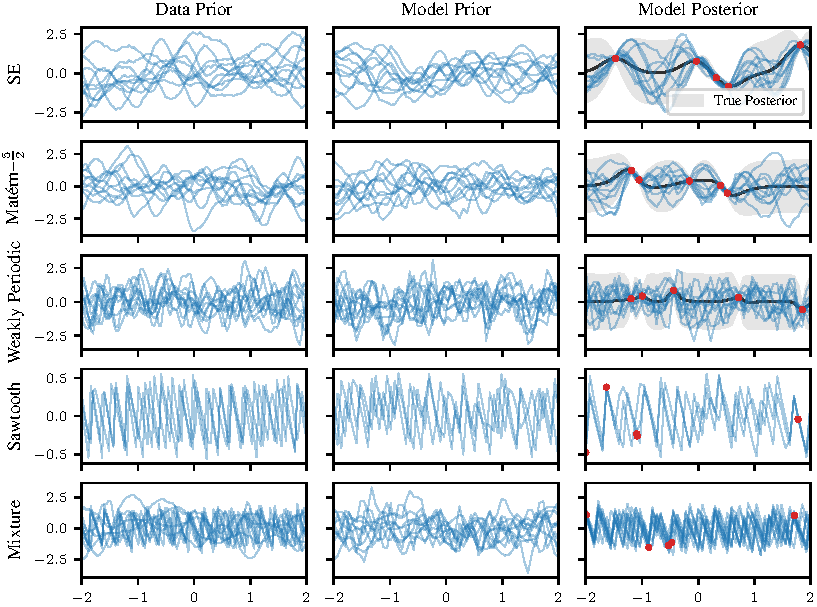
\includegraphics{images/geomndp/1d/plot_regression1d_appendix.pdf}
	\caption{Visualisation of 1D regression experiment.}
	\label{fig:app:regression}
\end{figure}

\begin{figure}
	\begin{subfigure}{\linewidth}
		\centering
		
\includegraphics{images/geomndp/1d/limiting_kernel_se_legend.pdf}\\\vspace{1mm}
		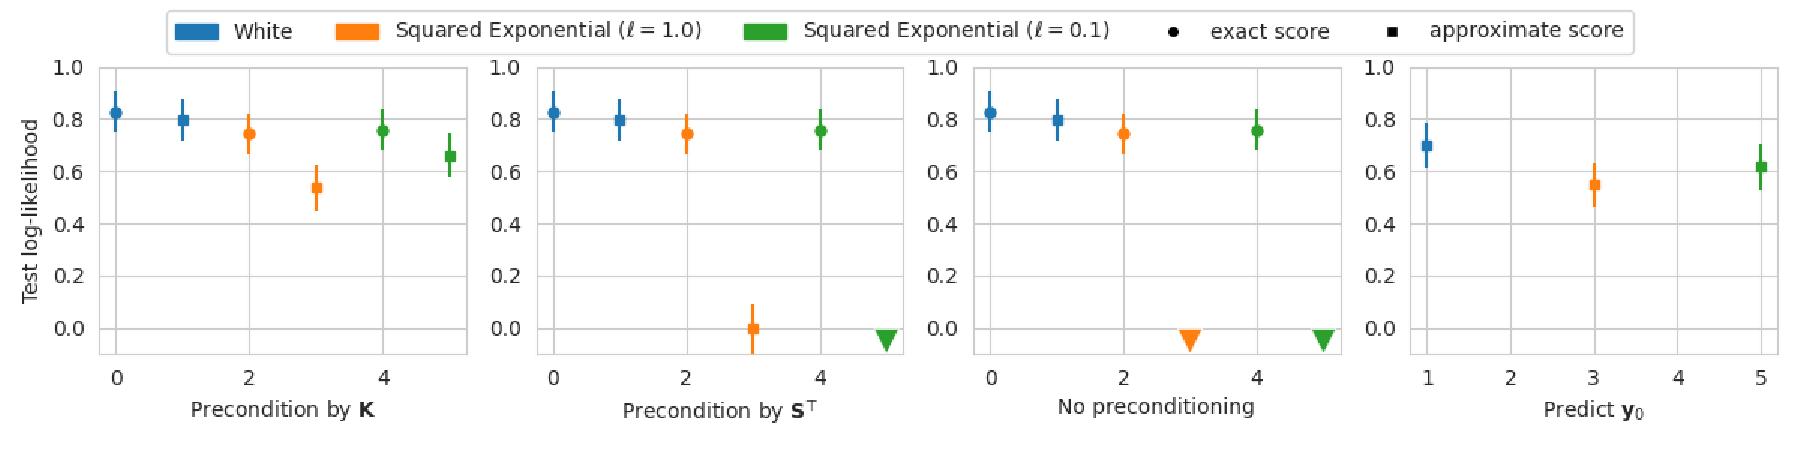
\includegraphics{images/geomndp/1d/limiting_kernel_se.pdf}
		\caption{Squared Exponential dataset with lengthscale $\ell=0.25$}
	\end{subfigure}
	\begin{subfigure}{\linewidth}
		\centering
		
\includegraphics{images/geomndp/1d/limiting_kernel_periodic_legend.pdf}\\\vspace{1mm}
		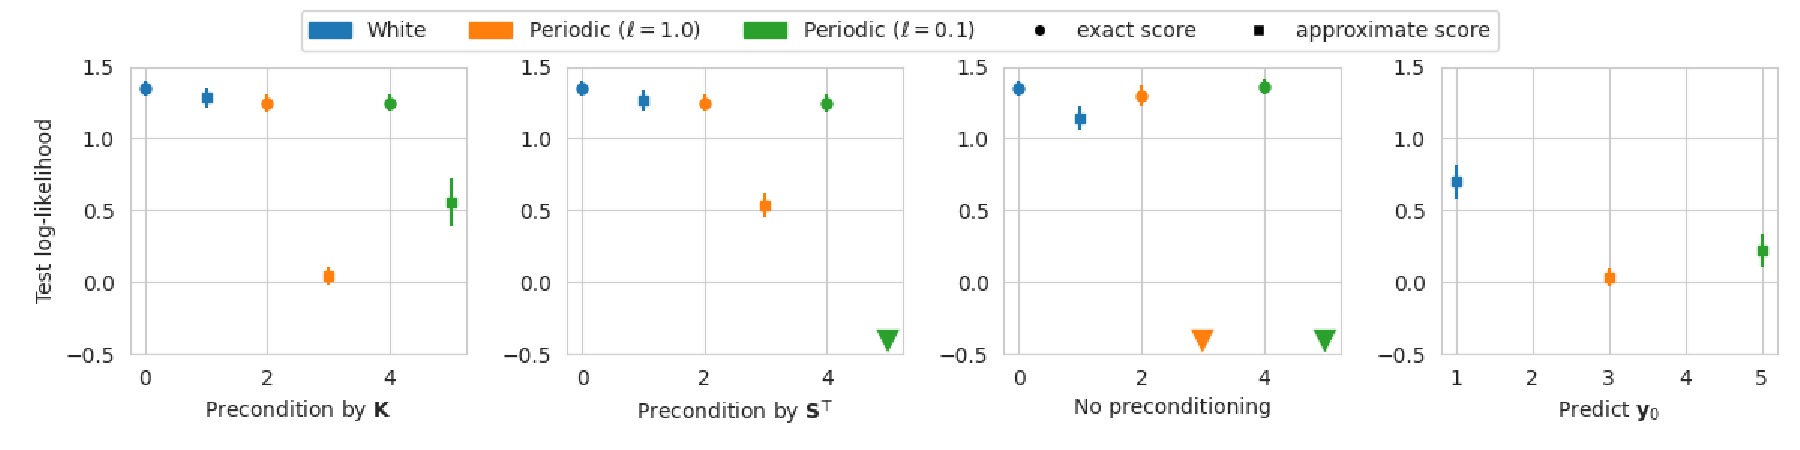
\includegraphics{images/geomndp/1d/limiting_kernel_periodic.pdf}
		\caption{Periodic dataset with lengthscale $\ell=0.25$}
	\end{subfigure}
	\label{fig:app:score-parametrization-ablation}
	\caption{\emph{Ablation study} targeting different limiting kernels and score parametrisations.}
\end{figure}

\begin{figure}
	\centering
	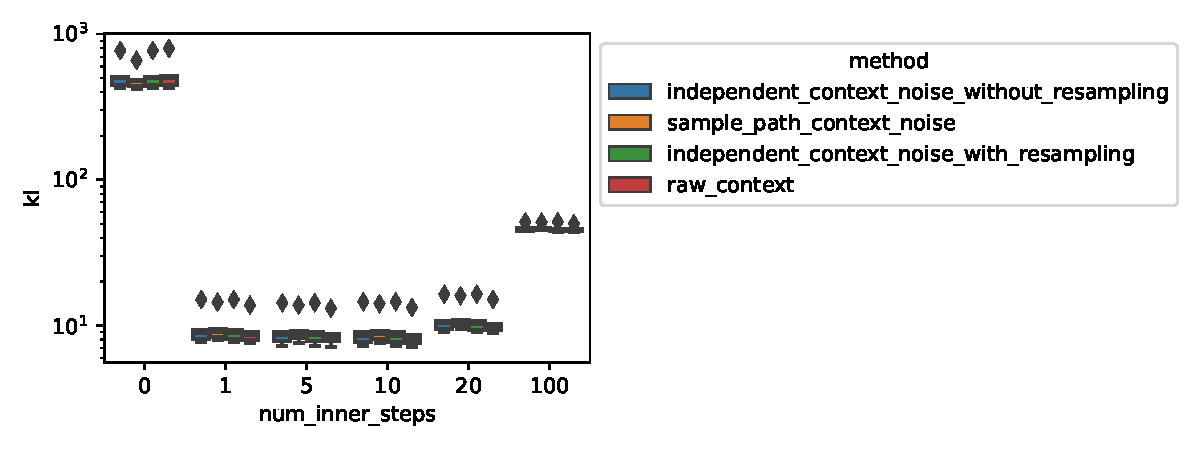
\includegraphics[width=\textwidth]{images/geomndp/1d/conditional_ablation.pdf}
	\caption{Ablation noising schemes for conditional sampling.}
	\label{fig:app:conditional-ablation}
\end{figure}

\subsection{Gaussian process vector fields}
\label{sec:app_vec_gp}

\paragraph{Data}
We create synthetic datasets using samples from two-dimensional zero-mean GPs with the following $\groupE{2}$-equivariant kernels: a diagonal Squared-Exponential ({\scshape SE}) kernel, a zero curl ({\scshape Curl-free}) kernel and a zero divergence ({\scshape Div-free}) kernel, as described in \cref{sec:en_equiv_kernels}.
We set the variance to $\sigma^2=1$ and the lengthscale to $\ell=\sqrt{5}$.
We evaluate these GPs on a disk grid, created via a 2D grid with $30 \times 30$ points regularly space on $[-10, 10]^2$ and keeping only the points inside the disk of radius $10$.
We create a training dataset of size $80\times10^3$.
and a test dataset of size $10\times10^3$.

\paragraph{Models}
We compare two flavours of our model GeomNDP \!
\!.
One with a non-equivariant attention-based score network \parencite[Figure C.1,][]{dutordoir2022Neural}, referred as {\scshape NDP\textsuperscript{*}}.
Another one with a $\groupE{2}$-equivariant score architecture, based on steerable CNNs~\parencite{thomas2018tensor,weiler20183Da}.
We rely on the \texttt{e3nn} library \parencite{e3nn_paper} for implementation.
A knn graph $\mathcal{E}$ is built with $k=20$.
The pairwise distances are first embed into $\mu(r_{ab})$ with a `smooth\_finite' basis of $50$ elements via \texttt{e3nn.soft\_one\_hot\_linspace}, and with a maximum radius of $2$.
The time is mapped via a sinusoidal embedding $\phi(t)$ \parencite{vaswani2017attention}.
Then edge features are obtained as $e_{ab} = \Psi^{(e)}(\mu(r_{ab})||\phi(t)) \ \forall (a, b) \in \mathcal{E}_k$ with $\Psi^{(e)}$ an MLP with $2$ hidden layers of width $64$.
We use $5$ \texttt{e3nn.FullyConnectedTensorProduct} layers with update given by $V_a^{k+1} = \sum_{b \in \mathcal{N}(a, \mathcal{E}_k)} V_a^{k} \otimes \left(\Psi^{v}(e_{ab}||V_a^k||V_b^k)\right) Y(\hat{r}_{ab})$ with $Y$ spherical harmonics up to order $2$m $\Psi^{v}$ an MLP with $2$ hidden layers of width $64$ acting on invariant features, and node features $V^k$ having irreps \texttt{12x0e + 12x0o + 4x1e + 4x1o}.
Each layer has a gate non-linearity \parencite{weiler20183Da}.

We also evaluate two neural processes, a translation-equivariant {\scshape ConvCNP} \parencite{gordon2019Convolutional} with decoder architecture based on 2D convolutional layers \parencite{lecungradient1998} and a $\mathrm{C}4 \ltimes \R^2 \subset \groupE{2}$-equivariant {\scshape SteerCNP} \parencite{holderrieth2021equivariant} with decoder architecture based on 2D steerable convolutions \parencite{weiler2021General}.
Specific details can be found in the accompanying codebase \url{https://github.com/PeterHolderrieth/Steerable_CNPs} of \textcite{holderrieth2021equivariant}.

\paragraph{Optimisation.}
Models are trained for $80k$ iterations, via \parencite{kingma2015Adam} with a learning rate of $5e-4$ and a batch size of $32$.
The neural diffusion processes are trained unconditionally, that is we feed GP samples evaluated on the full disk grid.
Their weights are updated via with exponential moving average, with coefficient $0.99$.
The diffusion coefficient is weighted by $\beta: \ t \mapsto \beta_{\min} + (\beta_{\max} - \beta_{\min}) \cdot t$, and $\beta_{\min}= 1e-4$, $\beta_{\max} = 15$.

As standard, the neural processes are trained by splitting the training batches into a context and evaluation set, similar to when evaluating the models.
Models have been trained on A100-SXM-80GB GPUs.

\paragraph{Evaluation.}
We measure the predictive log-likelihood of the data process samples under the model on a held-out test dataset.
The context sets are of size 25 and uniformly sampled from a disk grid of size $648$, and the models are evaluated on the complementary of the grid.
For neural diffusion processes, we estimate the likelihood by solving the associated probability flow ODE \eqref{eq:probability_flow_ode}.
The divergence is estimated with the Hutchinson estimator, with Rademacher noise, and 8 samples, whilst the ODE is solved with the 2nd order Heun solver, with $100$ discretisation steps.

We also report the performance of the data-generating {\scshape GP}, and the same GP but with diagonal posterior covariance {\scshape GP (Diag.)
	}.

\subsection{Tropical cyclone trajectory prediction}
\label{sec:cyclonedetail}

\textbf{Models. }

Four models were evaluated.

The \textsc{GP ($\R\to\R^2$)} took the raw latitude-longitude data and normalised it.
Using a 2-output RBF kernel with no covariance between the latitude and longitude and taking the cyclone time as input, placed a GP over the data.
The hyperparameters of this kernel were optimised using a maximum likelihood grid search over the data.
Note that this model places density outside the bounding box of $[-90, 90] \times [-180, 180]$ that defines the range of latitude and longitude, and so does not place a proper distribution on the space of paths on the sphere.

The \textsc{Stereographic GP ($\R \to \R^2/\{0\}$)} instead transformed the data under a sterographicc projection centred at the north pole, and used the same GP and optimisation as above.
Since this model only places density on a set of measure zero that does not correspond to the sphere, it does induce a proper distribution on the space of paths on the sphere.

The \textsc{NDP ($\R\to\R^2$)} uses the same preprocessing as \textsc{GP ($\R\to\R^2$)} but uses a Neural Diffusion Process from \cite{dutordoir2022Neural} to model the data.
This has the same shortcomings as the \textsc{GP ($\R\to\R^2$)} in not placing a proper density on the space of paths on the sphere.
The network used for the score function and the optimisation procedure is detailed below.
A linear beta schedule was used with $\beta_0=1e-4$ and $\beta_1=10$.
The reverse model was integrated back to $\epsilon=5e-4$ for numerical stability.
The reference measure was a white noise kernel with a variance $0.05$.
ODEs and SDEs were discretised with 1000 steps.

The \textsc{GeomNDP ($\R\to\c{S}^2$)} works with the data projected into 3d space on the surface of the sphere.
This projection makes no difference to the results of the model, but makes the computation of the manifold functions such as the exp map easier, and makes it easier to define a smooth score function on the sphere.
This is done by outputting a vector for the score from the neural network in 3d space, and projecting it onto the tangent space of the sphere at the given point.
For the necessity of this, see \cite{debortoli2021neurips}.
The network used for the score function and the optimisation procedure is detailed below.
A linear beta schedule was used with $\beta_0=1e-4$ and $\beta_1=15$.
The reverse model was integrated back to $\epsilon=5e-4$ for numerical stability.
The reference measure was a white noise kernel with a variance $0.05$.
ODEs and SDEs were discretised with 1000 steps.

\textbf{Neural network.}
The network used to learn the score function for both \textsc{NDP ($\R\to\R^2$)} and \textsc{GeomNDP ($\R\to\c{S}^2$)} is a bi-attention network from \textcite{dutordoir2022Neural} with 5 layers, hidden size of 128 and 4 heads per layer.
This results in 924k parameters.

\textbf{Optimisation. } \textsc{NDP ($\R\to\R^2$)} and \textsc{GeomNDP  ($\R\to\c{S}^2$)} were both optimised using (correctly implemented) Adam for 250k steps using a batch size of 1024 and global norm clipping of 1.
Batches were drawn from the shuffled data and refreshed each time the dataset was exhausted.
A learning rate schedule was used with 1000 warmup steps linearly from 1e-5 to 1e-3, and from there a cosine schedule decaying from 1e-3 to 1e-5.
With even probability either the whole cyclone track was used in the batch, or 20 random points were sub-sampled to train the model better for the conditional sampling task.

\textbf{Conditional sampling. }
The GP models used closed-form conditional sampling as described.
Both diffusion-based models used the Langevin sampling scheme described in this work.
1000 outer steps were used with 25 inner steps.
We use a $\psi=1.0$ and $\lambda_0=2.5$.
In addition at the end of the Langevin sampling, we run an additional 150 Langevin steps with $t=\epsilon$ as this visually improved performance.

\textbf{Evaluation. }
For the model (conditional) log probabilities the GP models were computed in closed form.
For the diffusion-based models, they were computed using the auxiliary likelihood ODE discretised over 1000 steps.
The conditional probabilities were computed via the difference between the log-likelihood of the whole trajectory and the log-likelihood of the context set only.
The mean squared errors were computed using the geodesic distance between 10 conditionally sampled trajectories, described above.
